\begin{savequote} ``In science there is only physics; all the rest is stamp collecting.''
\qauthor{Ernest Rutherford, 1st Baron Rutherford of Nelson}
\end{savequote}

\chapter{Introduction}

In this Chapter we review the subjects of jets and outflows in star formation,
introducing the theories and problems associated with gravitational collapse,
conservation of angular momentum and magnetocentrifugal launching of jets.
We discuss the rival theories for the launching of jets from young stars and the
role of shocks, give an overview of the derivation of the equations of
magnetohydrodynamics from the kinetic theory and outline the numerical methods
used for solving the magnetohydrodynamics equations. A survey of the history
and current state of star formation jet simulations is also presented.


%\newpage
%\minitoc
\section{Jets and outflows in nature}

% Matter exchange universe - general physical
% Star Fxn
% Collapse
% too much energy
% grav- kinetic
% outflows
% narrow fast outflows called jets
% Centre of present study
% techniques used
Matter does not remain stationary in the Universe, but moves and accelerates, driven by gravity and electromagnetic forces, collapsing into stars, exploding in supernova, streaming in jets and outflows. 
The interplay between the forces results in complex and often unexpected results. 
A good example of this may be seen in the large molecular clouds which pervade the galaxy, and collapse under the influence of gravity.
Surprisingly, inspection of the collapsing cloud reveals not just infalling matter but \emph{outflow}, in the form of narrow high-speed jets and wide-angle lower-speed molecular outflows.
% Outflows in AGN XRB GRB CV ONe YSO BD
Outflows appear to be ubiquitously linked with the process of accreting material onto a central mass. 
In fact, they are commonly found in observations of active galactic nuclei
(AGNs), brown dwarfs \citep{2005Natur.435..652W}, X-ray binaries, young stellar
objects (YSOs), planetary nebulae \citep[PN;][]{2006Natur.440...58V}, microquasars \citep{2002A&A...393L..99P}, 
%cataclysmic variables (CVs) 
and their presence is inferred in observations of gamma-ray bursts \citep[GRB;][]{2006A&A...455..423M}. 
They exist over a broad range of mass scales from the smallest brown dwarf jets with central objects of only a few tens of Jupiter masses to the monumental jets from AGNs which extend over thousands of parsecs from central objects with masses of over 100 million $M_{\odot}$.




\begin{table}
\begin{tabular}{|p{3.5cm}|p{4.5cm}|p{4.5cm}|}
\hline
& \emph{Length} & \emph{Central Mass} \\
\hline
AGN & 2,500 pc & $10^8 M_{sun}$ \\
\hline
YSO & 0.1 pc & $1 M_{sun}$ \\
\hline
BD & $<<$ 0.1 pc & $ 0.013 M_{sun}$ \\
\hline
\end{tabular}
\caption{The relative sizes of astrophysical jets}
\label{tab:jets}
\end{table}


Although the American astronomer Sherbourne Wesley Burnham observed a ``very small condensed nebula'' near to the young star T Tauri in 1890, 
the first observation of an astrophysical jet proper was that of
Heber Doust \citet{1918PLicO..13...55C} who described a ``curious straight ray ... apparently
connected to the nucleus by a thin line of matter'' near the spiral galaxy M87. 
This research is primarily focussed on jets and outflows in the star formation process.
These have been observed in the form of chains of emitting nebulae first separately observed by
\citet{1951ApJ...113..697H} and \citet{1952ApJ...115..572H}.
The nebulae were named Herbig-Haro objects (or HH objects) in their honour.  
\citet{1958PASP...70..399O} suggested that the HH objects might be related to
mass-loss caused by rotation of the T Tauri star. 
\citet{1975ApJ...195..631S} tabulated the forbidden-line emission ratios of an
object in Burnham's Nebula (now called HH255) against those of a supernova remnant and was able to conclude that the
line ratios could only be produced by a radiative shock. While it was originally
speculated that the shock was caused by an ionised wind striking a small
cloudlet \citep{1978ApJ...223..884S},
it was soon realised that the convexity of the bow shock implied a directed flow
impinging on an ambient medium. The chains of visible Herbig-Haro knots were
originally attributed to crossing shocks in the jet \citep{1987MNRAS.225..741F}, but are now considered much
more likely to be induced by velocity variations in the outflow \citep{2001A&A...367..959R}.


\begin{figure}[t]
\centering
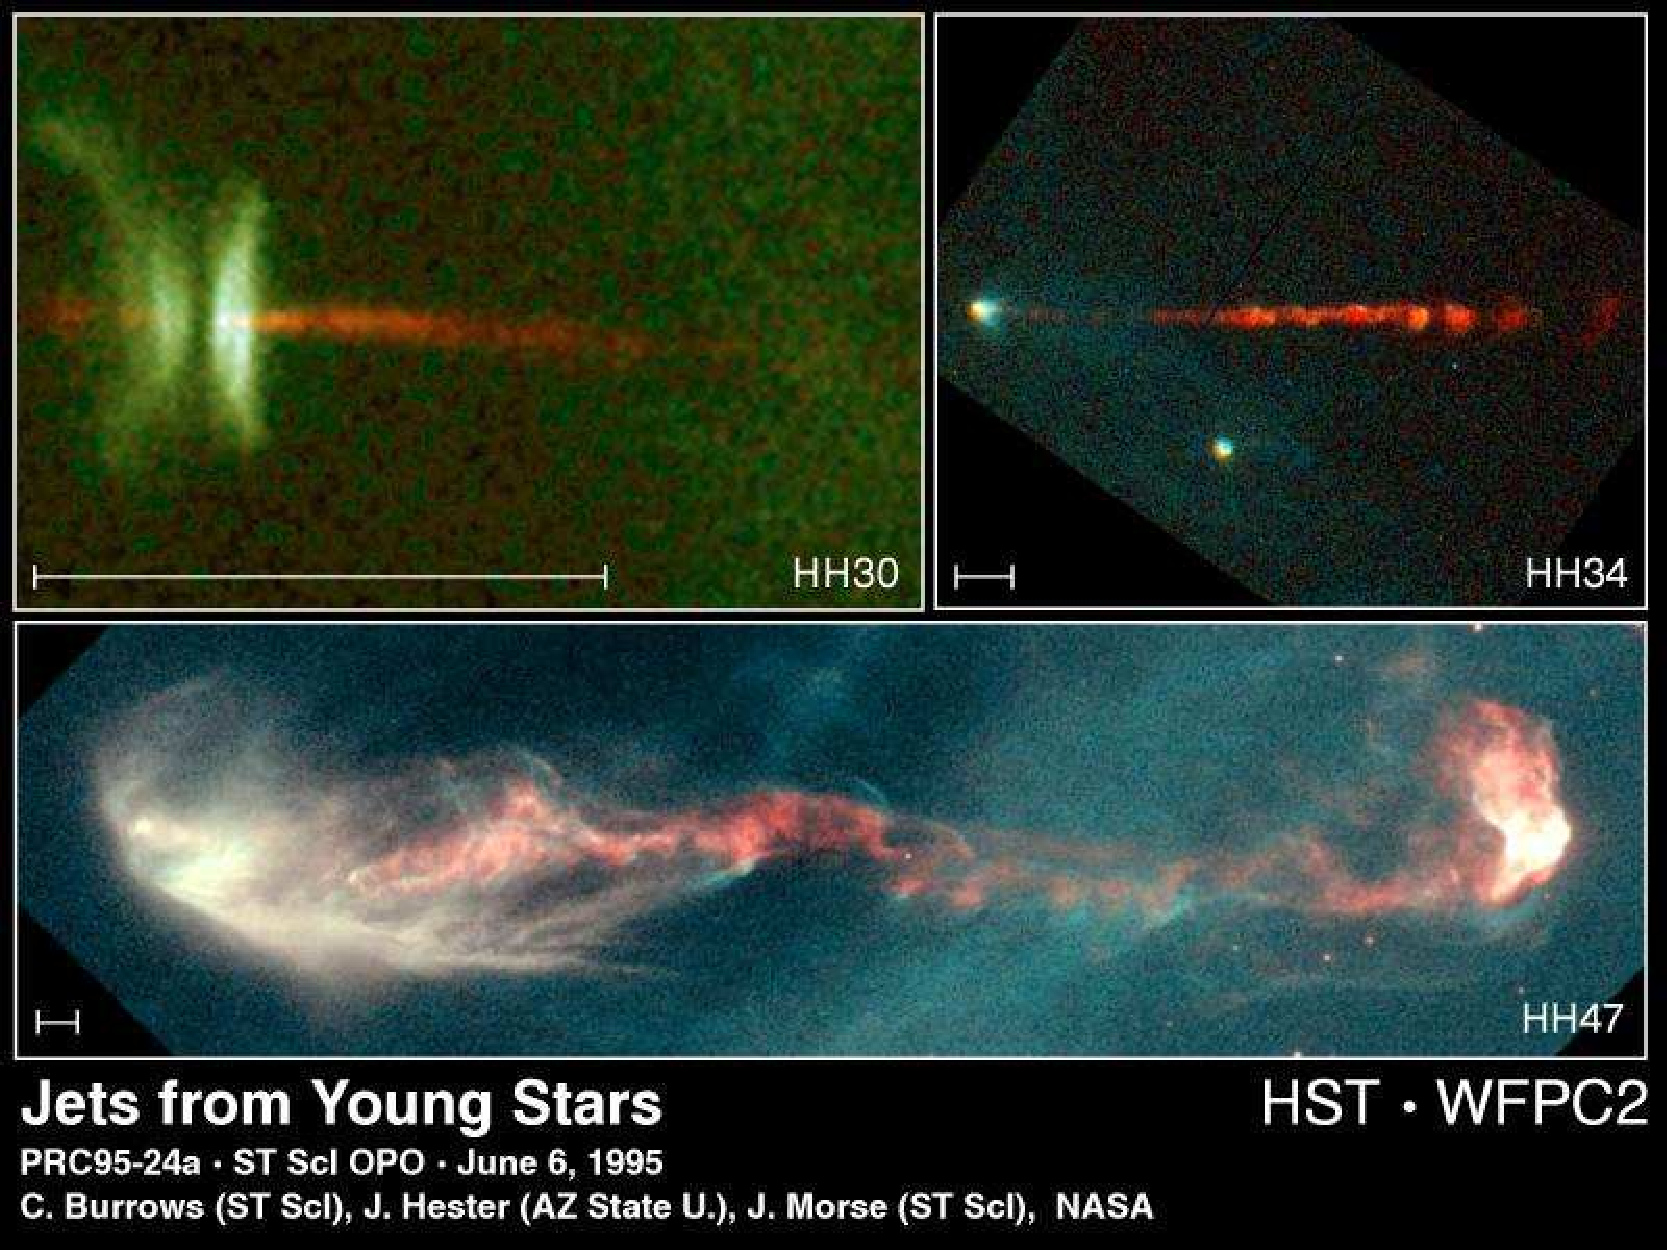
\includegraphics[width=\textwidth]{protostellar_jets}
\caption{
Jets from young stellar objects at different ages.
Chains of Herbig-Haro knots, jet wiggling, and the terminal bow shock are all visible.
Upper Left Credit: C. Burrows (STScI, ESA), the WFPC 2 Investigation Definition Team, and NASA
Upper Right Credit: J. Hester (Arizona State University), the WFPC 2 Investigation Definition Team, and NASA
Bottom Credit: J. Morse/STScI, and NASA.
}
\label{fig:jet} % label
\end{figure}



%%%%%%%%% STAR FORMATION %%%%%%%%%%%%%%%%%%%%%
\section{Jets and star formation}

% How do stars form
%goal is to understand star formation and how matter in a cloud condenses into a molecular cloud core and thence into a protostar.
% How does matter accrete


\subsection{Gravitational collapse mediated by magnetic fields and turbulence}
The modern theory of star formation has its origins in the nebular hypothesis of
\citet{kant:55} and \citet{laplace:96}.
According to current understanding, a star
% Nebular hypothesis
begins life in a rotating molecular cloud, made up of mainly ($\sim$99\%)
molecular hydrogen and helium and dust. 
Giant molecular clouds may be observed in molecular lines (such as H$_{2}$~1-0~S(1)), 
21cm hydrogen and optically thanks to reflected either light from nearby stars.
They can also be seen in extinction maps in silhouette against light from background stars.
The dust component plays a vital role in star formation, allowing material to
cool down both by blocking light from other nearby stars (extinction) and by adsorbing
hydrogen and onto grain surfaces and thereby catalysing the formation of molecular
hydrogen, further cooling the molecular cloud \citep{1979ApJS...41..555H}.
In Chapter 6 the extinction property of dust is exploited to produce maps of the
dust clouds in the Galactic plane.



\begin{figure}[t]
\begin{center}
 \begin{minipage}[c]{.48\linewidth}
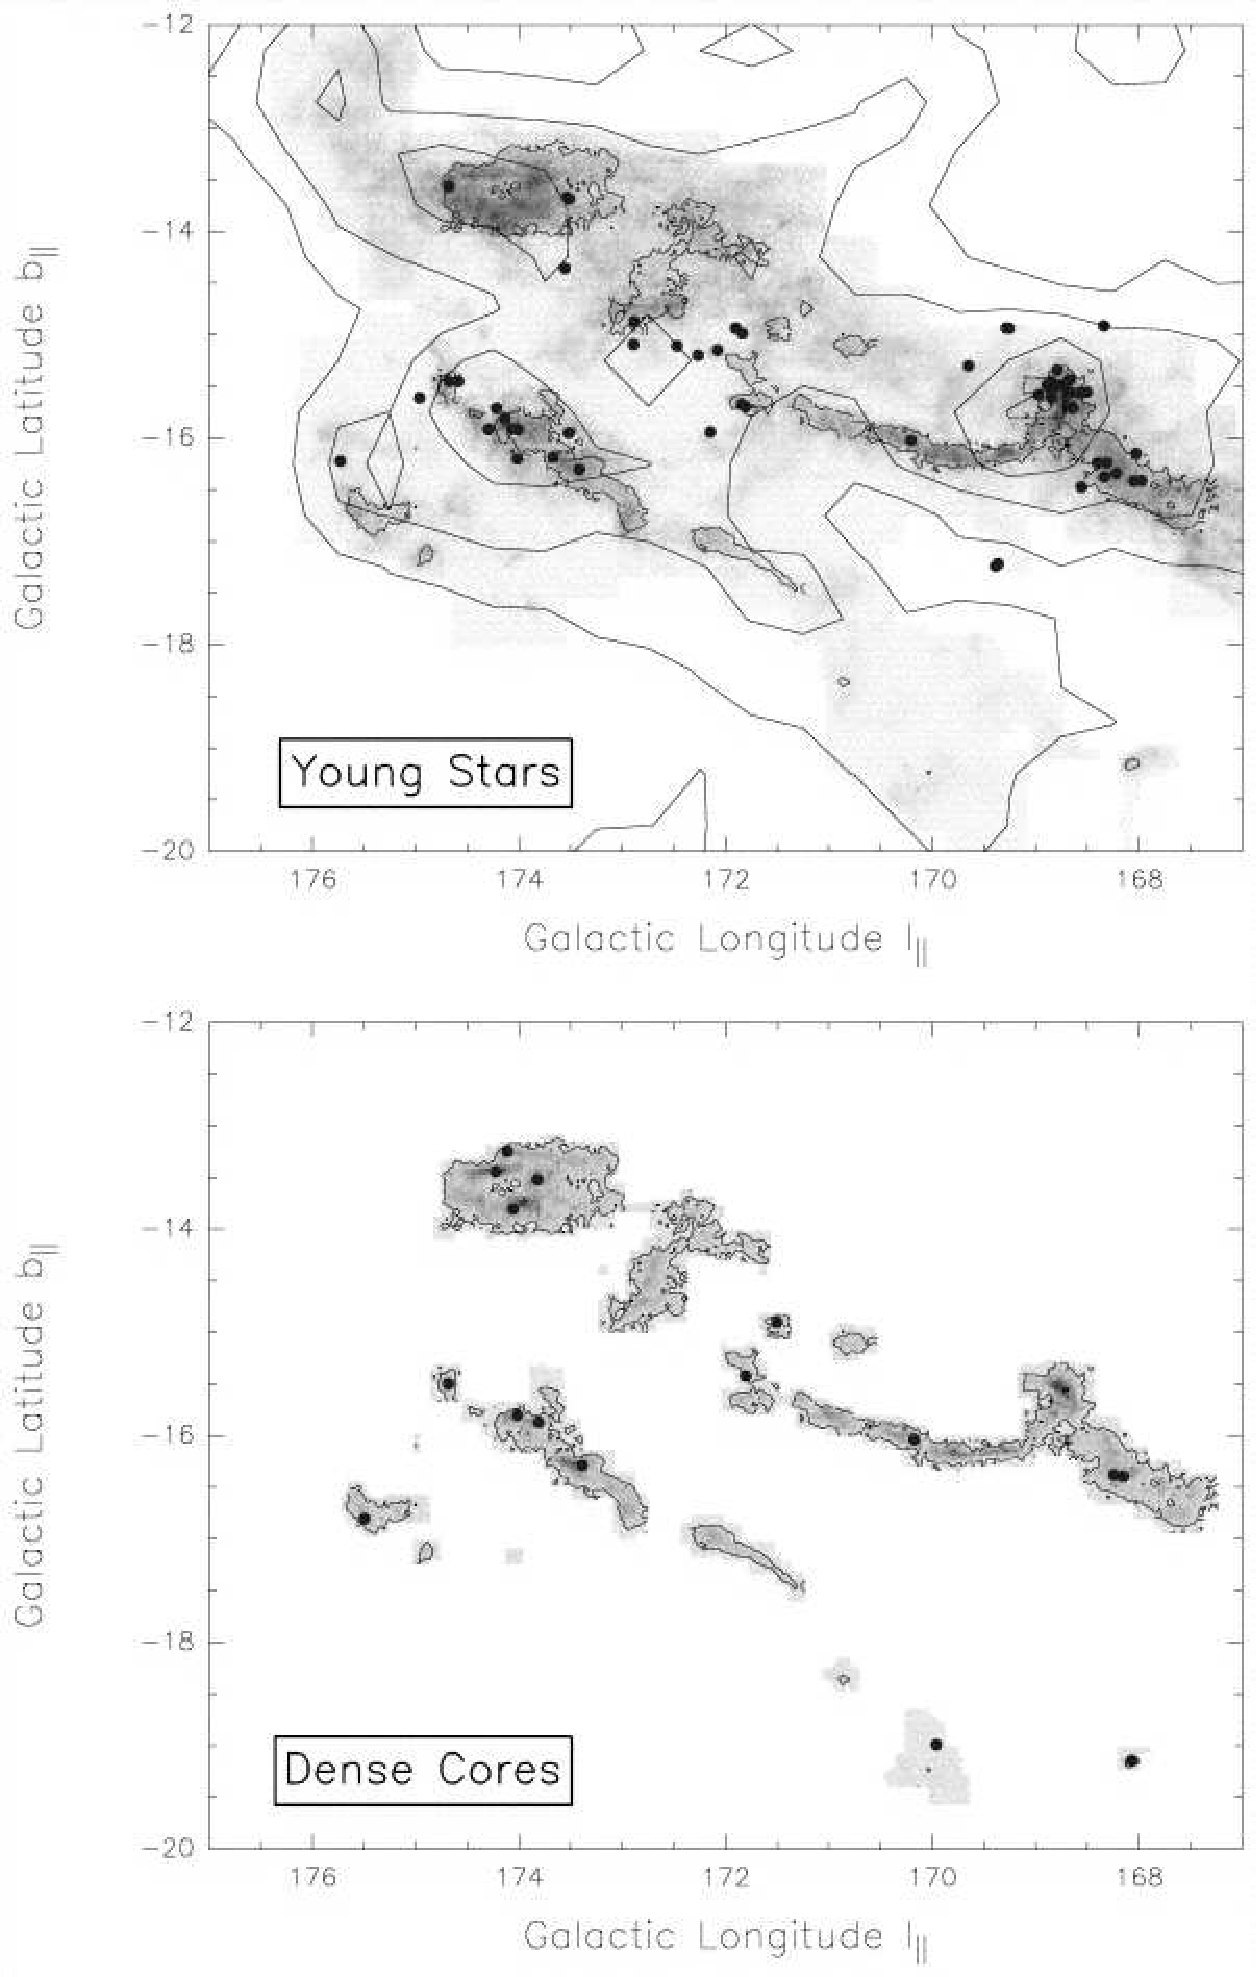
\includegraphics[width=5cm]{taurus}
 \end{minipage} \hfill
 \begin{minipage}[c]{.48\linewidth}
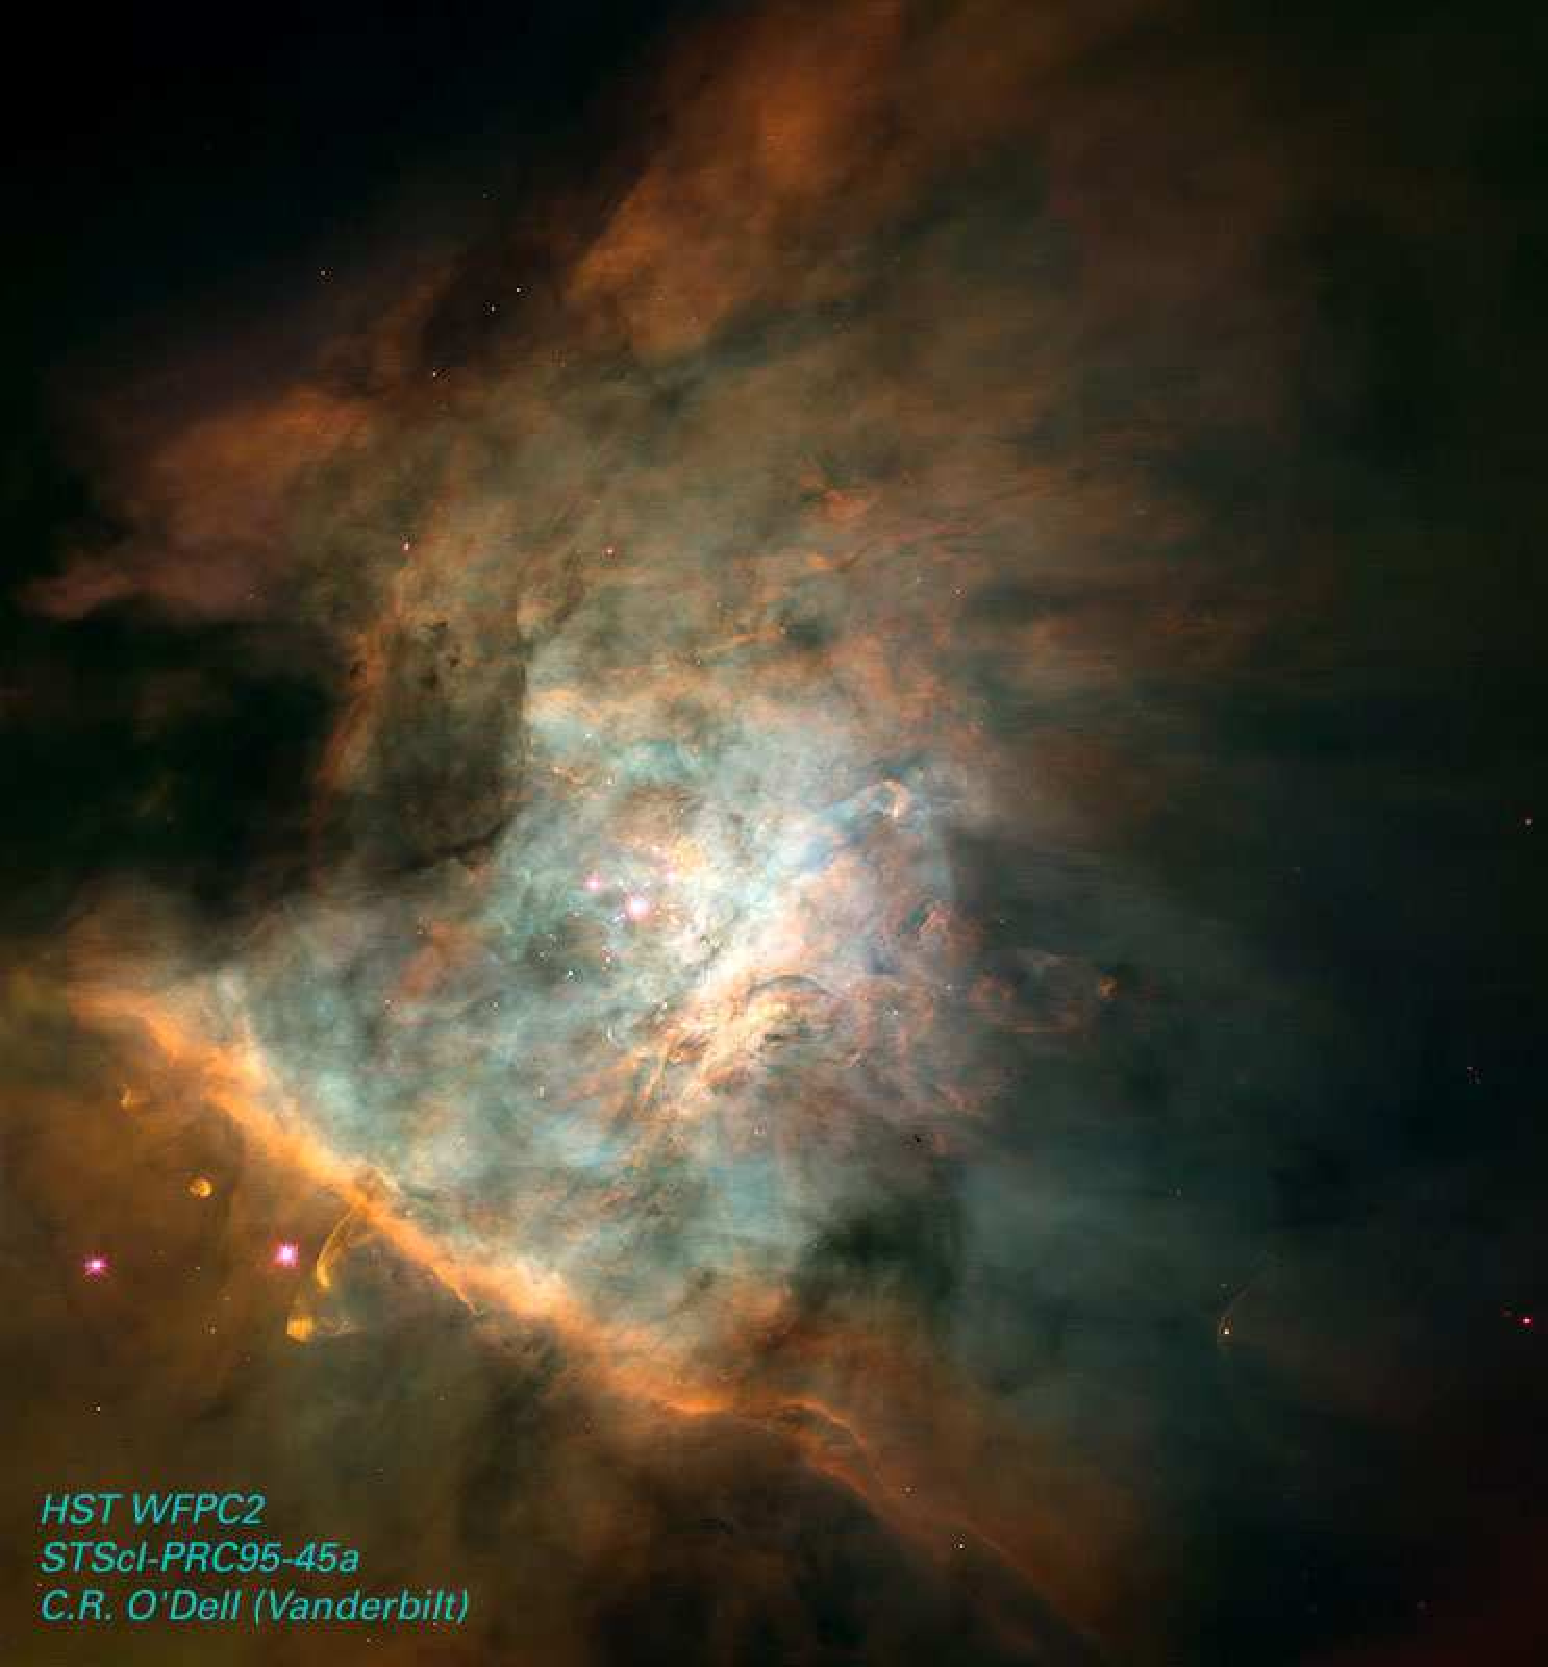
\includegraphics[width=5cm]{molecular_cloud}
 \end{minipage} \hfill

\caption{
Left panel:
Taurus-Auriga giant molecular cloud in $^{13}CO$.
Right panel: Star formation region: the Orion Nebula ( NGC 1976, M42) - a 2.5 light-year section of the giant molecular cloud and star-formation region in Orion.
The colour composite image shows oxygen in blue, hydrogen in green and nitrogen in red - atomic lines generated by reflection from nearby main sequence and massive stars.
Image from NASA, C.R. O'Dell and S.K. Wong (Rice University).
}
\label{fig:gmc} % label
\end{center}
\end{figure}

Giant molecular clouds are thought to be supported against gravitational
collapse by a seemingly formidable coalition of
thermal pressure, ambient magnetic fields and turbulence, but over time the turbulence can
dissipate, and the cloud can become prone to condensing into clumps and
subsequently cores when
neutral matter is drawn together by the gravitational force and slips unaffected
through the magnetic field lines in the process known as ambipolar diffusion. 
Such cores can be observed in molecular line emission and the submillimetre continuum.
The process of
condensation may also be triggered or accelerated by interactions from supernova
remnants or jets and outflows, which create irregularities in the density
structure of the molecular cloud \citep{1997MNRAS.285..201B}.
% Jeans mass, gravitational runaway and collapse 
% Disk forms 
When matter builds up in a pressure-supported dense core it will
eventually reach the Jeans mass\footnote{
 The Jeans mass, $M_J \approx {c_s}^3 / \left( G^{3/2} {\rho}^{1/2} \right)$, where $c_s$ is the sound speed, $G$ , the Universal Gravitational Constant, and $\rho$ is the average density.
It is derived by equating the freefall time $t_{ff} \simeq /\sqrt{G\rho} $ to the sound wave crossing time $t_{cross}=R/c_s$.
%The derivation of the Jeans mass relies on the so-called ``Jeans swindle'' which simplifies the problem of gravitational collapse by unphysically assuming the environment around the collapsing object is not also collapsing.
}, $M_J$. 
$M_J$ corresponds to the limit of gravitational stability beyond
which the cloud will start to collapse.
The gravitational collapse will not be a pure free-fall but will be slowed by the magnetic field
and turbulence.
The infalling matter possesses an inherent angular momentum, and therefore will not in general precipitate directly on the small central
object, but will instead distribute itself around
the centre of gravity in the equatorial plane, forming a disk of matter typically rotating
at Keplerian speeds very close to the centre of gravity.
Such disks were originally inferred from the infra-red excess visible in the
spectra of young stars, which implied some distribution of material about the
central object, arranged so as not to obscure the young star completely. \citet{1993ApJ...410..696O} used the Hubble Space Telescope to produce the first images of the predicted disks.


%\begin{figure}[t]
%\centering
%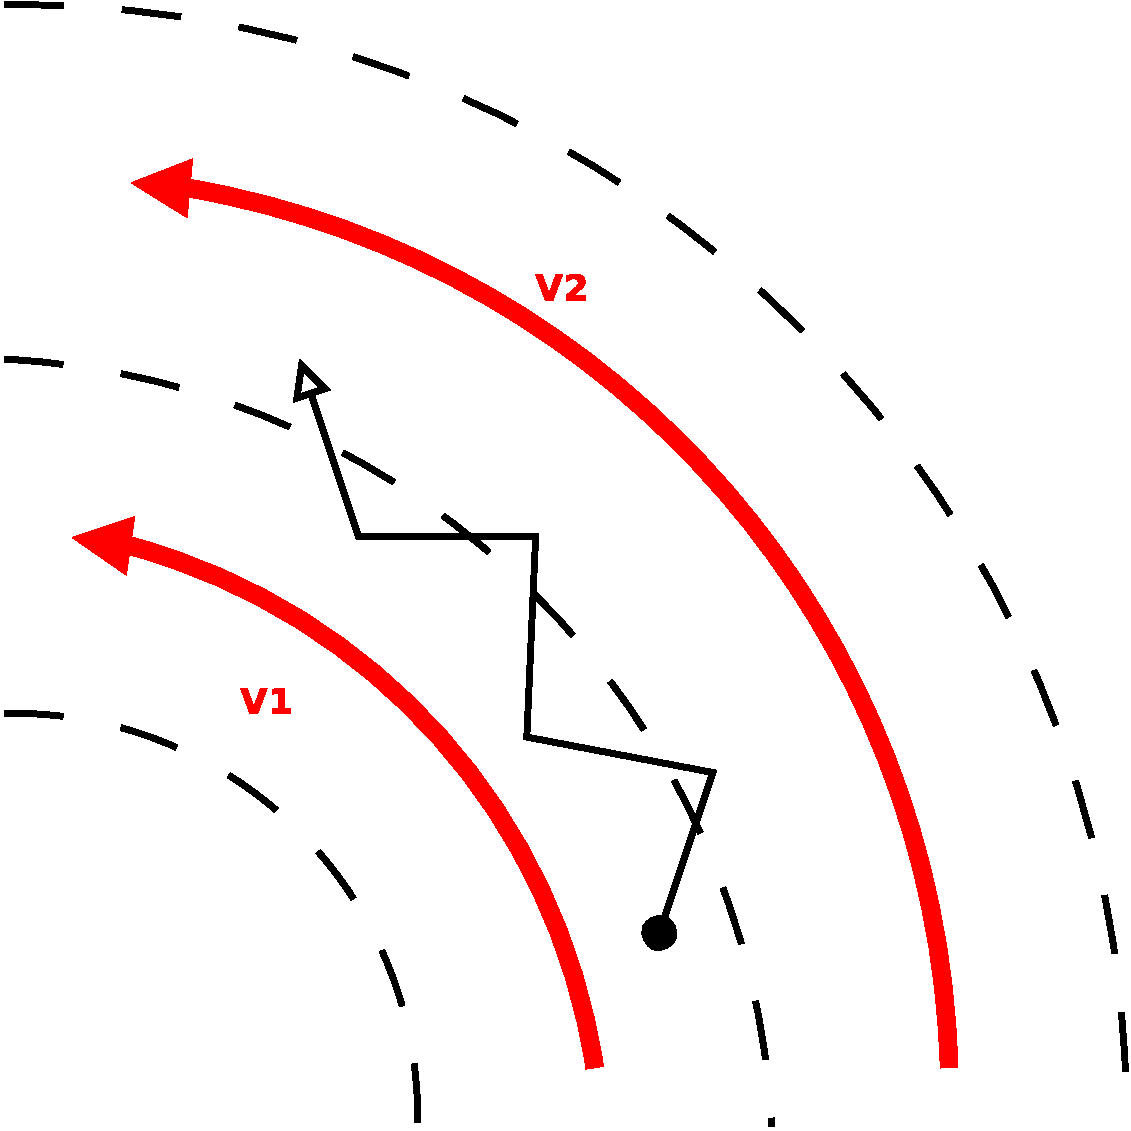
\includegraphics[width=2cm]{MyViscousDisk}
%\caption{Differentially rotating disk annuli: The random thermal movement of gases in between the annuli results in collisions and transfer of angular momentum. After a collision the inner particle transfers momentum to the outer particle and gravitates inward, the outer particle has increased its energy and moves outward.  }
%\label{fig:ViscousDisk} % label
%\end{figure}

% Viscosity
%The differential rotation of the fluid annuli generates shear viscous forces.
% These viscous flows have a sufficiently high Reynolds number for turbulence to
% set in.
%Due to the random thermal motion of the gas particles (Figure \ref{fig:ViscousDisk}), there is a net transfer of angular momentum outward.
The rotating disk possesses an effective viscosity, the cause of which is still unknown, but may be due to the Balbus-Hawley (Magnetorotational) Instability \citep{1991ApJ...376..214B} generating turbulence in the disk .
The more slowly moving material in the disk will gradually spiral inward and accrete onto the protostar, as long as it has velocity lower than the escape/break-up velocity of the protostar.
%Material at the corotation radius will either be ejected from the surface in an outflow.
% What role do magnetic fields play
% Accretion columns via magnetic field lines
If the protostar is magnetised the material inside the radius of the
magnetosphere may accrete onto the protostar via the magnetic field lines.
These columns of accreting material will generate shocks at their bases which
may be detected as hot spots on the surfaces of accreting protostar.
Fields in the range of a few kilogauss on the surface of a protostar have been observed \citep{1993PASP..105..955H}.
The role of turbulence is still an open question but it may tangle the magnetic
field lines, transport angular momentum out of the disk and slow down the cloud
collapse.

\subsection{Angular momentum problem}
% The angular momentum problem
Due to the conservation of angular momentum $m \omega r^2$, the angular velocity, $\omega$
will tend to increase, in order to compensate for the decrease in radius, $r$ as the core collapses.
\citet{1985ApJ...293..216P} points out that observed accretion disk
specific angular momenta ($\sim$ 10$^{22}$ cm$^2$ s$^{-1}$) are much greater that those for formed stars ($\sim$ 10$^{17-18}$ cm$^2$ s$^{-1}$).
%The infalling matter then possesses an \emph{angular momentum excess} that must be transported away if the star is to continue accreting matter, otherwise the fast-rotating material will spin up the protostar and cause it to reach break-up velocity, at which point the gravitational force is insufficiently strong to continue acquiring matter and the process of accretion will draw to a halt.
%
% In order to account for the observed great decrease in angular momentum some means of transporting the angular momentum excess out of the disk is necessary.
%
Indeed if all the angular momentum from the condensing cloud was conserved
within the sytem it would lead to ``ridiculous spin rates''
\citep{1974MNRAS.168..603L}).
A mechanism is thus required to transport angular momentum out of the star-disk
system.
Angular momentum transport can be achieved through the \emph{deflection} of infalling material into highly collimated jets or molecular outflows that are associated with protostars and young stars.
% One angular momentum transport mechanism is through the highly collimated jets or molecular outflows which are visibly associated with the young stars.
Other mechanisms include the transfer of angular momentum from rotation to
orbital motion (fragmention into a binary or multiple star), or transport of angular momentum
outwards through the disk by turbulent viscosity (\citet{1943ZA.....24..181V},
\citet{1952ZN.....34..263L} and
\citet{1974MNRAS.168..603L}).
% Also Lust 1952 von Weizsacker 1943


\subsection{Magnetocentrifugal launching}

\begin{figure}[t]
\centering
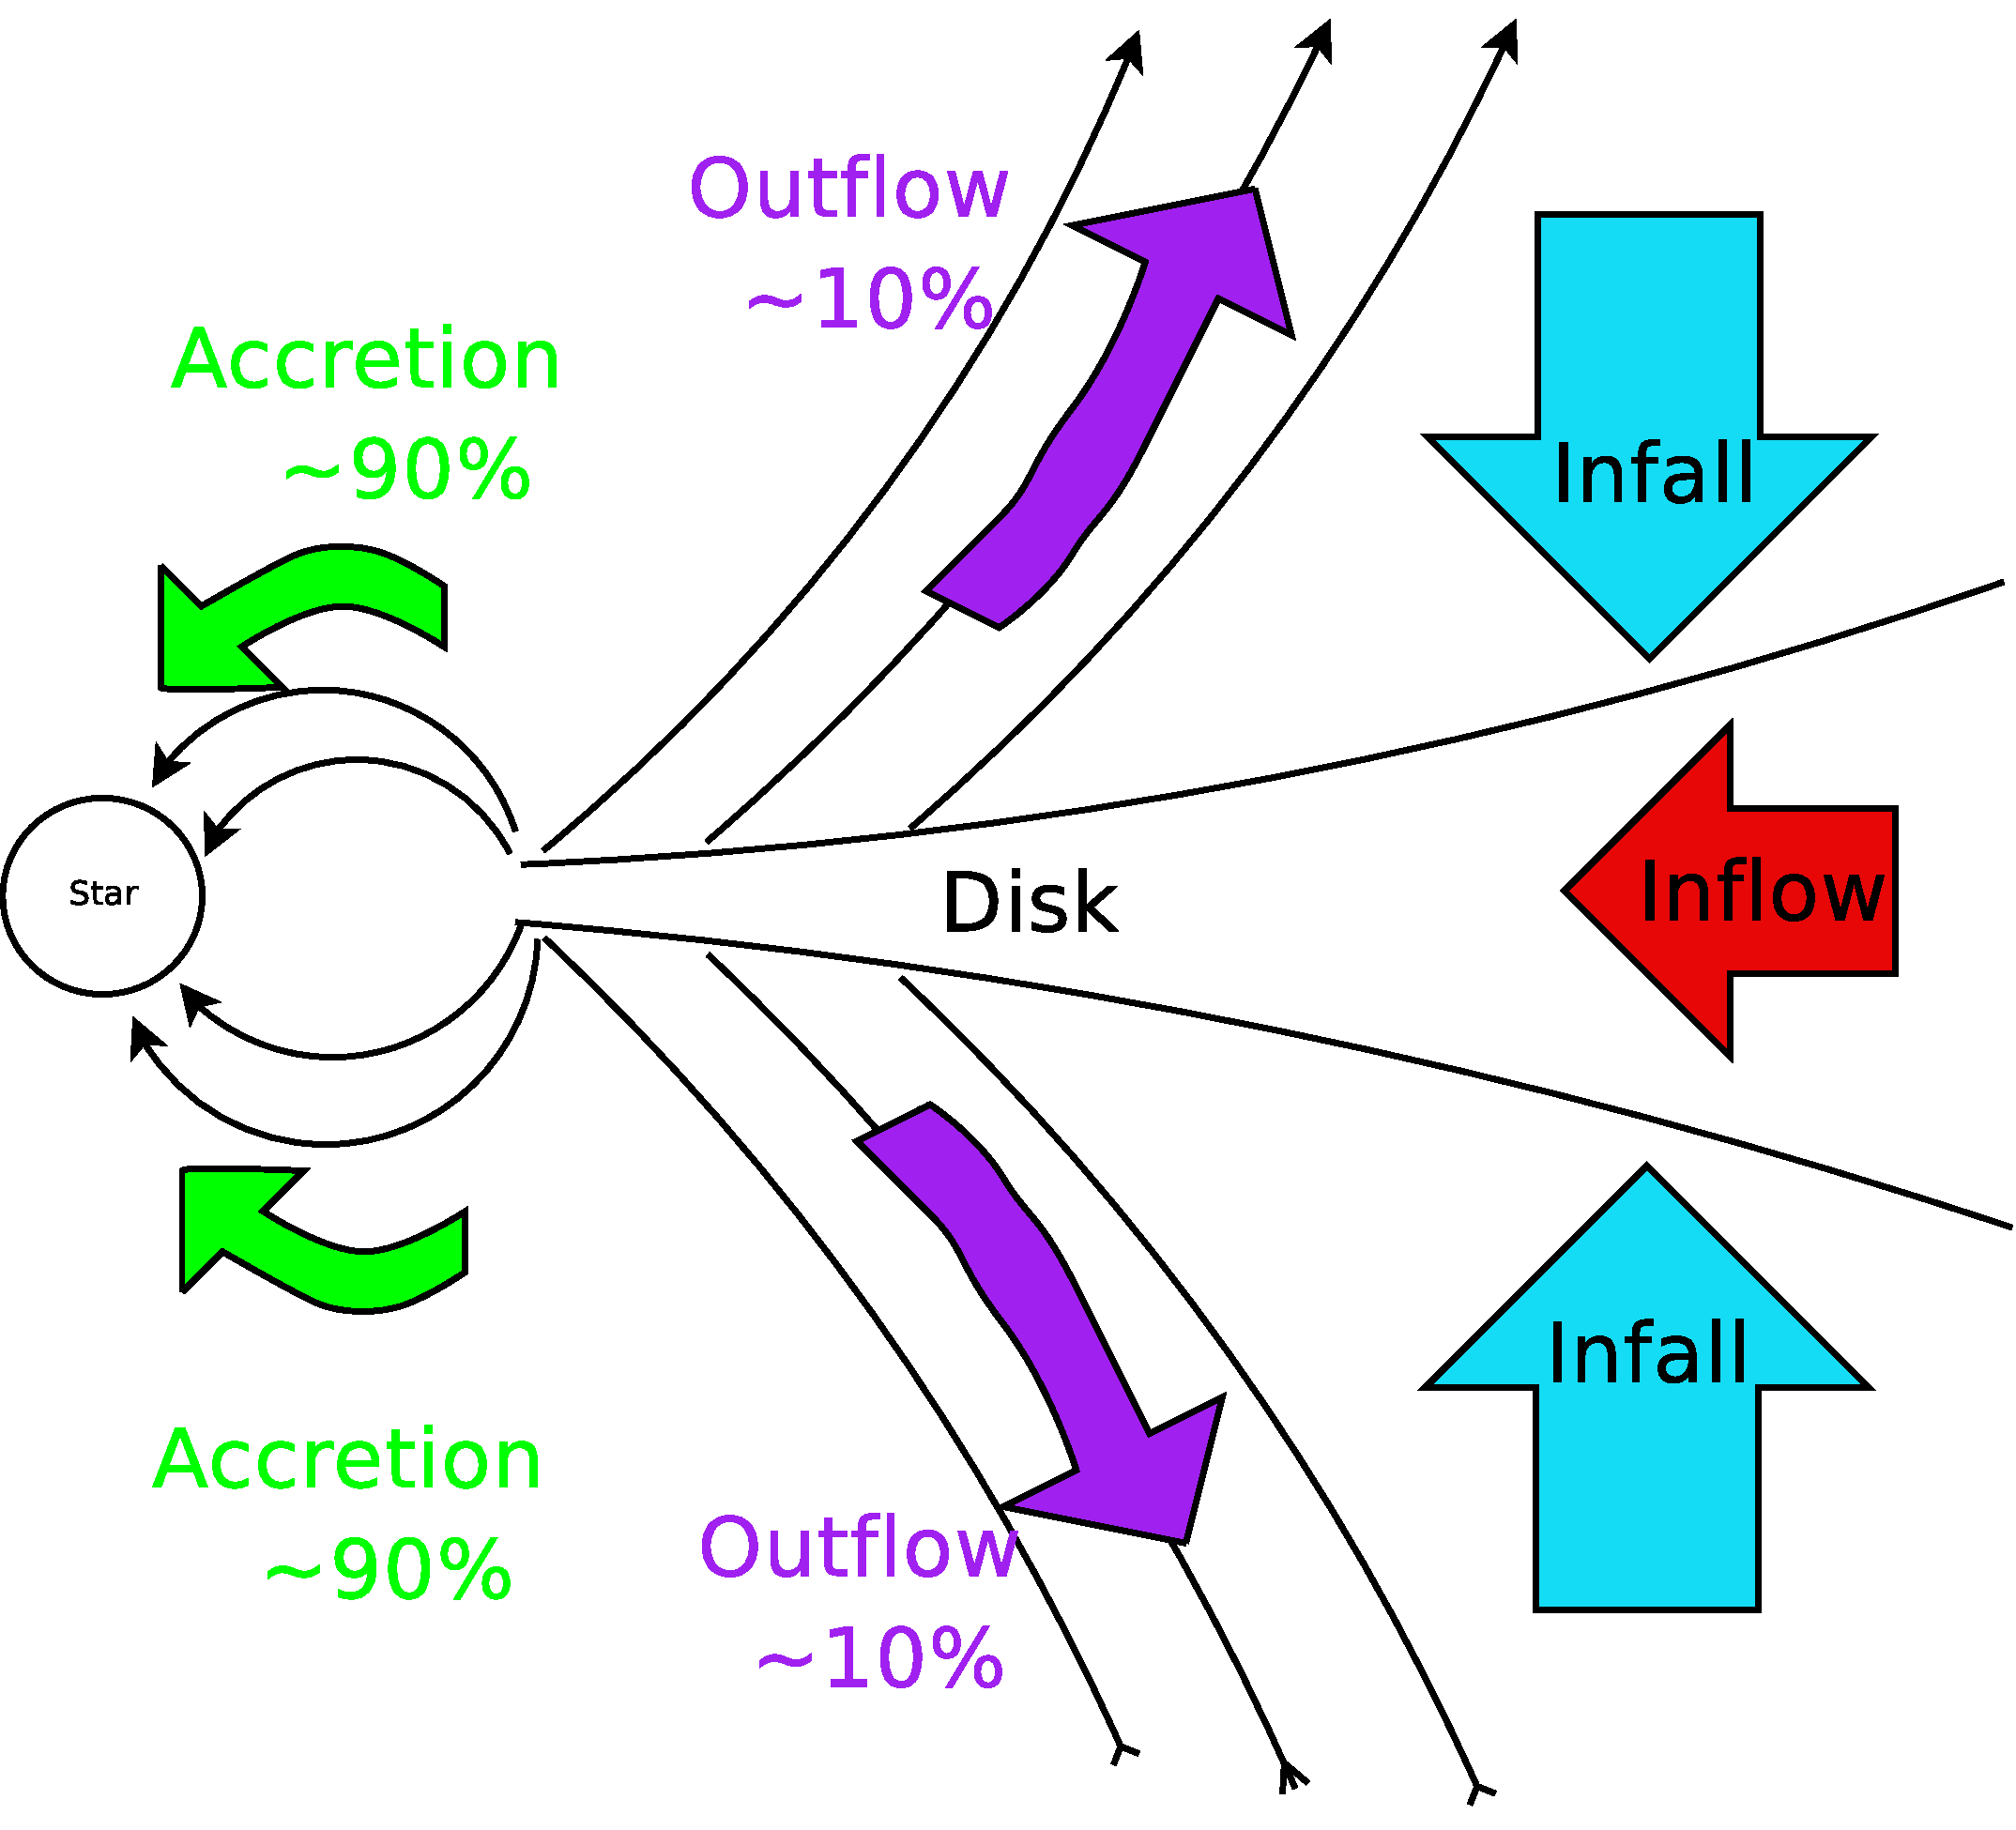
\includegraphics[width=0.8\textwidth]{MagneticSlingshot}
\caption{
Schematic of the star-disk-outflow configuration. Typically $\sim$90\% of the infalling material is accreting onto the star, carrying $\sim$10\% of the angular momentum. The 10\% not accreted will be flung off in an outflow, carrying 90\% of the angular momentum.
%The right panel shows 3d view of the disk and magnetic field lines.
}
\label{fig:MagneticSlingshot} % label
\end{figure}

% Magnetic slingshot
% bead on-a-wire
Rotating matter can be flung out from the polar regions of the disk like a
magnetic slingshot and will preferentially travel along magnetic field lines
like beads strung on a wire \citep{1971MNRAS.152..323H} while slower moving matter continues to accrete onto the protostar.
The flow of accreting and outflowing material is sketched in Figure \ref{fig:MagneticSlingshot}.
% Alfv\a'{e}n radius
The cylindrical column of material which makes up the outflowing material will
be bound to the disk by the magnetic field lines which thread it and will
therefore corotate with it up to the Alfv\a'{e}n surface.
(The Alfv\a'{e}n surface is defined as the surface at which the ram pressure of
the outflowing  material equals the magnetic pressure and the fluid is able to bend the magnetic field line.
If the magnetic field is a dipole 
$\mathbf{B}=\frac{\boldsymbol{\mu}}{r^3}$
(where $ \boldsymbol{\mu}$ is the magnetic moment)
one can derive a closed-form expression for
the Alfv\a'{e}n radius. 
Balancing the ram and magnetic pressures:
$
\rho v^2 = B^2 = \frac{\mu^2}{r^6}
$
one gets
$
r_A= \left( \frac{\mu^2}{\rho v^2}\right)^\frac{1}{6}
$
.
The dipole approximation is not necessarily valid for the whole star-disk region.
)
% Back torque
% Magnetic braking
The outflowing material will, by applying a back torque, magnetically brake the disk, enough to allow collapse. (More angular momentum can be removed by the viscosity in the accretion disk as mentioned previously.)

\subsection{Binary Star Formation}
%\textcolor{red}
%{
Although the above theories feature a cloud collapsing to form a single star, 
\citet{1991A&A...248..485D},
\citet{1992ASPC...32...73M},
\citet{1992ASPC...32...50Z},
\citet{1993AJ....106.2005G},
\citet{1995ApJ...443..625S},
\citet{1999NewA....4..531P}, have studied multiplicity and found frequent examples of binarity. 
%Notwithstanding some dissent on this point, see \citet{2006ApJ...640L..63L}, binary stars are commonly found, especially in star forming regions.
The binary formation mechanism, whether by fragmentation of a molecular core or capture of a nearby star by gravity must therefore be efficient.
In Chapter \ref{BinaryJetsChap} the role played by binary jets in the star formation process is explored.
%}


%\cleardoublepage
%\pagebreak
\begin{figure*}[th]
\centering
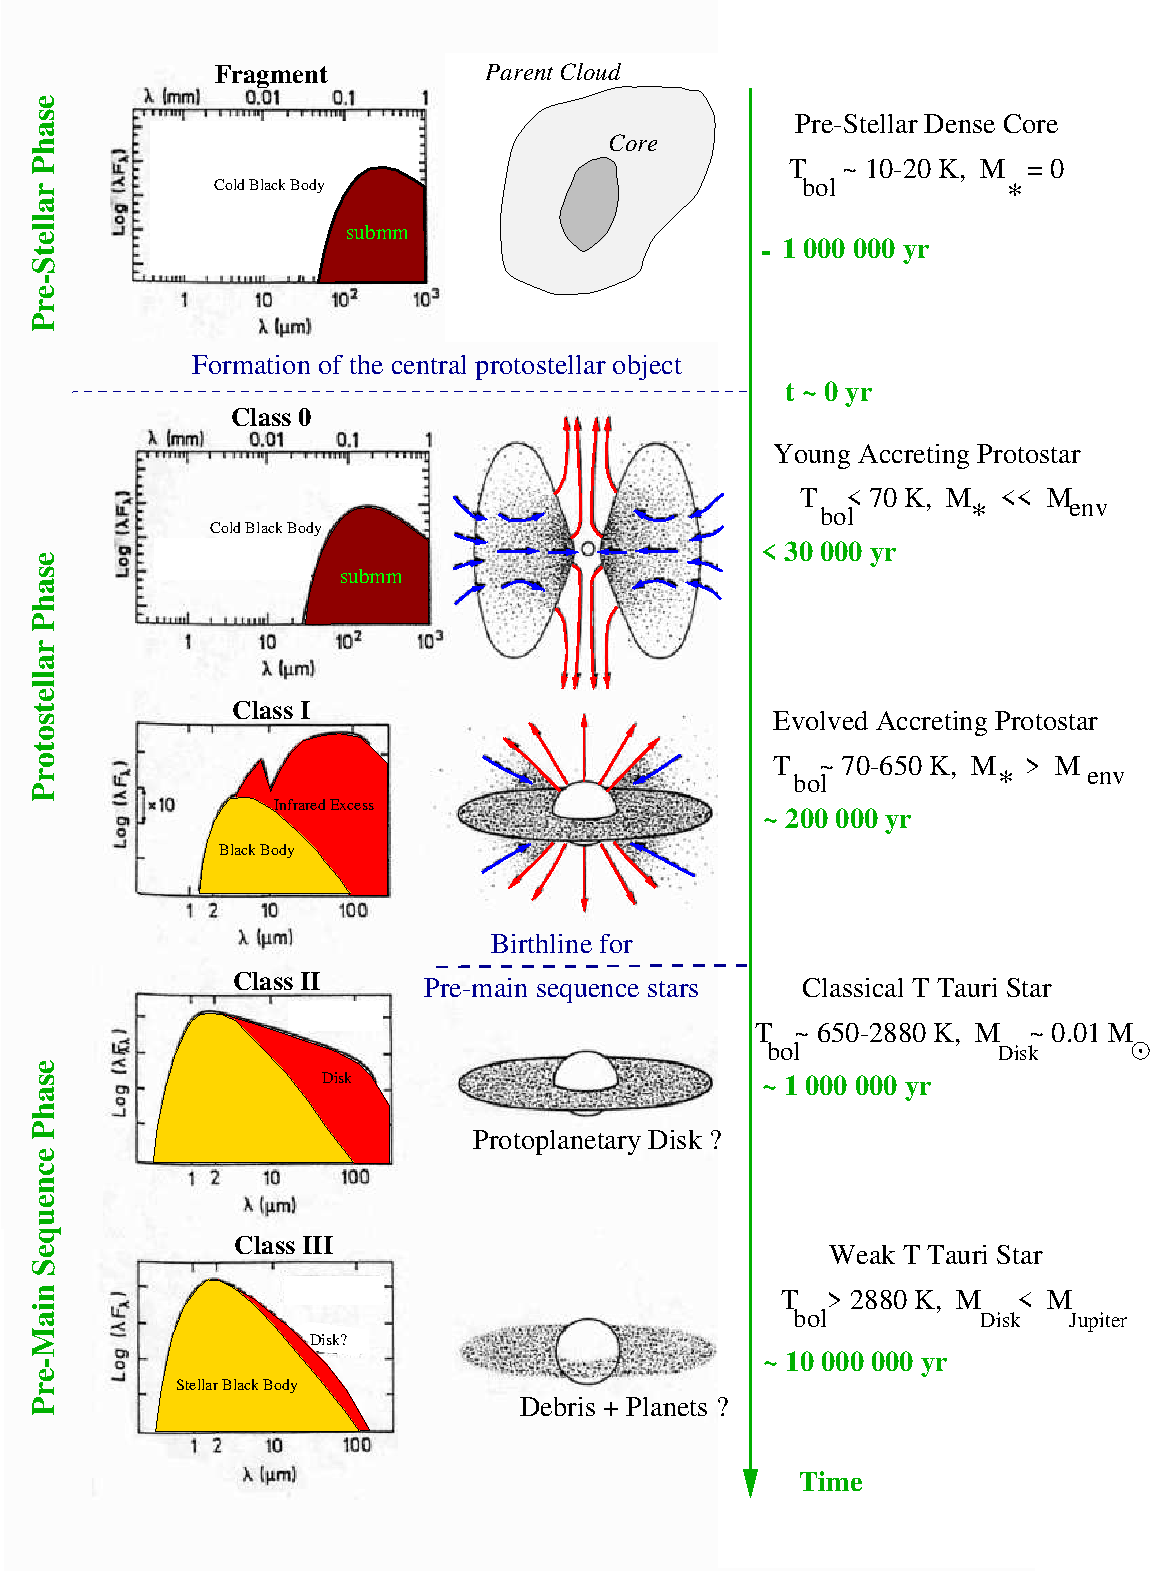
\includegraphics[width=14cm]{evolution}
\caption{ Classification of low mass protostars according to their spectral energy
density and their bolometric temperature \citep{1993ApJ...406..122A}. The temperature increase is seen in the movement of the spectrum down the
wavelength axis. 
The excess of infrared was deduced by observers to be some material distributed around the star in such a way as not to completely block it out. 
The presence of a disk was surmised. 
%Protostellar disks were first imaged using the Hubble Space Telescope.
}
\label{fig:1-1} % label
\end{figure*}
%\pagebreak
% ********** THIS MAY HAVE TO BE REMOVED ****************
% ********** THIS MAY HAVE TO BE REMOVED ****************
% ********** THIS MAY HAVE TO BE REMOVED ****************
% ********** THIS MAY HAVE TO BE REMOVED ****************
% ********** THIS MAY HAVE TO BE REMOVED ****************
\clearpage
\newpage
% *******************************************************

\subsection{Empirical Classification for Low Mass Stars}
Observers have classified low-mass young stellar objects according to their spectra.
This classification
\citep{1987IAUS..115....1L,1993ApJ...406..122A} is depicted in Figure \ref{fig:1-1}.
The scheme is consistent with an evolutionary sequence, increasing in time from Class 0 to Class III.
The first stage corresponds to Class 0 objects, the most deeply embedded sources. 
Such objects are still surrounded by infalling envelopes containing at least half of the mass of the central object. 
All Class 0 objects are associated with highly collimated molecular outflows, typically more
energetic than those associated with the next stage, i.e. Class I objects. 
The latter are still deeply embedded in dense envelopes and not optically visible. 
They are often associated with jets and molecular bipolar outflows, though less energetic than those associated with Class 0 objects.
Jets are highly collimated (opening angles of $\sim$ 1$^{\circ}$ - 5$^{\circ}$,
radii of $\sim$ 0.001 pc - 0.05 pc), denser than the ambient medium (densities $\sim$ 10$^2$ - 10$^3$~cm$^{-3}$) beams of matter travelling at high speeds ($\sim$ 200~km~s$^{-1}$) which plough through the interstellar medium. 
Molecular outflows are more dense ($\sim$ 10$^4$ - 10$^6$~cm$^{-3}$), less well-collimated flows with wider opening angles. 
Typical values for the jet and outflow parameters are shown in Table \ref{tab:mytable}.
Class II objects, or Classical T-Tauri stars, are surrounded by an accretion disk but with no infalling envelopes. 
Finally, Class III objects (weak T-Tauri stars) have a photo-sphere with a
radial stellar wind although free of any significant amounts of circumstellar material.
% Supersonic speed and shocks
The outflowing material is either supersonically launched or accelerated up to supersonic speeds very rapidly.
% Back to jets all of a sudden
Jets propagate at supersonic and super-Alfv\'enic speed and in doing so they shock the gas in the
ambient medium ahead, forming a bow shock. 
Additionally if the velocity of the jet is episodically varied at the source the jet will form
internal shocks or working surfaces where the slower moving material meets the faster moving
material.
The resulting emission, highly visible in optical wavelengths, paradoxically the result of an outflow, is the main source of information to the earthbound observer about the accretion process which mainly consists of infall.
In this study models are of jets from a Class I type protostar which are in general atomic, fast, less dense and narrow. Class 0 outflows are typically heavy, dense, slow, and molecular.


\subsection{High-Mass Stars}

% from web:
% Massive star formation takes place in clusters, in conditions which are both crowded and confused. Despite its luminosity, which enables a complete census of massive star formation to be undertaken in the galaxy, it is still a poorly understood process. This is because of the many interacting phenomena associated with it, for which it is hard to disentangle cause and effect, and the short timescale on which they occur. Indeed, the radiation pressure generated by a massive protostar, once it has reached 10 Msun, would seem sufficient to be able to halt any further accretion, so it remains a mystery how higher mass stars are formed at all. It has even been suggested that massive stars form via coalescence of lower mass (< 10 Msun) stars, inside exceedingly dense cluster environments. If so, they do so at stellar densities that have not been probed yet. Several developments have occurred recently which provide new tools for the study of massive star formation. Mid-IR imaging cameras are now available on the 8-m class optical/IR telescopes, equipped with a suite of filters for working between 8-30µm. Their diffraction limited observations provide an order of magnitude gain in speed over capabilities of 4-m class telescopes. The interaction of the young stars with their molecular clouds is also probed by a variety of spectral lines in the thermal-IR. Associated phenomena include masers, particularly water and methanol masers, which provide clear signposts to the presence of massive star formation across the galaxy. It is not clear what their direct association with star formation is, however. Are the masers in disks around embedded sources, sites where shocks are interacting with molecular gas, or simply fortuitous sight lines through hot molecular cores? Interferometry allows not only the relative location of masers and embedded sources to be ascertained, but also the structure within groups of maser spots. 
%
%



%\textcolor{red}
{
High-mass star formation is even less well understood than low-mass star formation.
Massive stars form in crowded clusters, riddled with multiple outflows and supernova remnants.
A major problem with the theory is how high mass protostellar objects overcome the radiation pressure, which counteracts the gravitational force and in principle could halt the process of accretion \citep{1974A&A....37..149K, 1977A&A....54..183Y, 1987ApJ...319..850W}.
%The radiation pressure is thought to exert a limit of approximately 20 solar masses , whereas 
Radiation pressure is thought to prevent stars of $>$ 20 solar masses (depending on the model) from forming, whereas
stars of up to 100 solar masses have been observed \citep{2004ApJ...610L.109F}.
%and the progenitor of the supernova 1961v in NGC 1058 is estimated at about 1000 solar masses.
Massive stars have much shorter lives than low-mass stars, many different phenomena are present and occur on short timescales.
O stars are deeply embedded for 15\% of their lifetimes which makes them hard to observe \citep{1989ApJ...340..265W}.
Observations of such dusty regions are restricted to longer wavelengths.
All or nearly all forming stars show strong outflows \citep{1989ApJ...340..472T}.
Observational difficulties are compounded by the fact that massive stars are relatively rare and the nearest massive star-forming region is 500 parsecs away in Orion.
One theory of high-mass star formation is competitive accretion, somewhat endearingly termed the ``nurture, not nature'' scenario, where the amount of accretion is related to the number of neighbours \citep{2004MNRAS.349..735B}.
Another theory is the coalescence scenario, where low mass stars collide to form massive stars, avoiding the radiation pressure limit \citep{1998MNRAS.298...93B}.
Another school of theories concentrates on quantative adjustments of the standard low-mass star formation theory.
It is also possible to increase the amount of material accreted if the radiation pressure or the accretion is anisotropic \citep{2006ApJ...637..798C}.
See \citet{Beutheretal2006} for a review.
}

\begin{table}
%\begin{tabular}{|p{4cm}|p{6cm}|}
\begin{tabular}{|p{3.5cm}|p{4.5cm}|p{4.5cm}|}
\hline
& \emph{Jet} & \emph{Molecular Outflow}
\\
\hline
Velocities:& 50-400 km/s (1) & 10-50 km/s
\\
\hline
Density: &10$^{2}$ -10$^{3}$ cm$^{-3}$ (2) & 10$^4$ - 10$^5$ cm$^{-3}$
\\
\hline
Length: & 0.1~pc - 10~pc (3) & 10$^4$ AU
\\
\hline
Radius: & 0.01~pc - 0.5~pc (3) & 
\\
\hline
Temperature:& 10$^{3}$-10$^6$K &  10-10$^4$K 
\\
\hline
Tracer materials:& [HI], [NII],[OI], [SII] & CO, H$_2$,
SiO$_3$
\\
\hline
Opening Angle: &1$^\circ$-10$^\circ$ (3) & 5$^\circ$-40$^\circ$
\\
\hline
\end{tabular}
\caption{Typically observed parameters for jets and molecular outflows associated with Class I protostars \protect\\1. \citet{2000prpl.conf..815E},\protect\\2. \citet{1999A&A...342..717B},\protect\\3. \citet{1996PhDT........56D} }
\label{tab:mytable}
\end{table}
% No indent ???


\section{Rival jet launching theories}
%How jets are generated}

%It is generally believed, based on a very great deal of correlating observational evidence, that accretion powers outflows and jets under the influence of magnetic fields.
Although the major models for the generation of jets agree on the magnetocentrifugal origin of the jets - they diverge on other points.
Following \citet{1996ARA&A..34..111B}, the current models for jet generation can be subdivided into two main categories, disk-driven winds and boundary-layer driven winds.

\subsection{Stellar winds}

% Parker wind
Very early analytical models by \citet{1958ApJ...128..664P} were successful at explaining and predicting the velocity of the solar wind using a purely one-dimensional spherically symmetric hydrodynamic thermally driven wind.
However this theory cannot explain the directional, collimated nature of the protostellar jets.
Including the magnetic field in the analysis \citep{1967ApJ...148..217W} makes the wind directional.
In fact it is not thought possible that highly collimated jets originate from protostellar surfaces.
\citet{1996ARA&A..34..111B} gives several reasons why jets cannot originate from central stars.
\begin{itemize}
\item Neutral species observed at high velocities around YSOs suggest the origin of the wind could not be at the hot stellar surface.
\item To drive a jet the star would need to rotate at or near breakup velocity - much faster than the observed T Tauri rotation speeds.
\item There is a strong correlation between presence of jets and presence of disks for young stellar objects.
\end{itemize}
For these reasons it is thought that the jet origin is not at the central source but either in the disk or at the boundary layer.
% Read bachiller and get the reasons.



\begin{figure}[th]
\centering
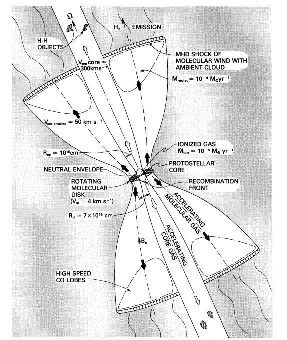
\includegraphics[width=7cm]{pudritz86}
\caption{
The Disk Wind Model, the jet is magnetocentrifugally launched from a broad region in the disk (Figure from \citet{1980ApJ...239L..17S}).
}
\label{fig:DiskWind} % label
\end{figure}

\subsection{Disk-driven winds}
Several theories of jet formation of varying degrees of credibility exist.
\citet[][; herafter BP82]{1982MNRAS.199..883B} in a seminal paper were responsible for an early jet generation model, originally devised for extragalactic jets but later applied to YSO jets by \citet{1983ApJ...274..677P,1985ApJ...293..216P,1986ApJ...301..571P} and \citet{1989ApJ...342..208K}.
BP82 imagined an external magnetic field threading a disk.
If the poloidal component of the magnetic field makes an angle less than
60$^{\circ}$ from a rotating disk, the centrifugal force can fling a packet of gas off the surface of the disk to infinity.
This may be visualised using the mechanical analogy suggested by \citet{1971MNRAS.152..323H} of a bead on a rigid massless wire attached to a rotating disk. 
If the wire is normal to the plane of the disk the bead will not move.
If it makes an angle less than a critical angle to the disk the bead will move up the wire.

The magnetic field threading the disk is analogous to the wire, pinched in at the centre by an accretion disk (see Figure \ref{fig:DiskWind}) which provided a bead-on-a-wire mechanism for the packets of gas to transport angular momentum away from the protostellar disk.
The packet of gas will be launched at escape velocity, and accelerated up to the typical outflow velocity by the magnetic field.
In their steady-state model, BP82 did not account for the time variations in velocity which appear to be the cause of several observed Herbig-Haro objects.

\citet{1985PASJ...37..515U} performed the first numerical simulations of the disk winds, modelling the accretion disk's rotation twisted the field as well as the disk's contraction compressing and strengthening the field until powerful reconnection events occur leading to an episodic outflow burst. At this point the field lines are straight, normal to the disk and the cycle begins again.

\citet{1995MNRAS.275..244L} discussed differential rotation causing loop inflation and opening of the field lines - allowing an outflow along the opened field lines. However, this is a steady flow model and does not account for episodic outflows.
\citet{1997ApJ...489..199G,1999ApJ...524..142G,1999ApJ...524..159G} modelled differential rotation causing loop inflation resulting in reconnection releasing jet plasma from the system. This model is capable of producing an unsteady flow with knots.

% Disk wind weaknesses

The weaknesses of the disk-driven wind theory centre on the magnetic field.
The required field in the disk has to be maintained by a turbulent dynamo but this is expected to be too weak.
The external fields in the disk are possibly insufficient to launch the wind.
\citet{2002ApJ...574..232M,2004ApJ...607L..43M,2005MNRAS.356..167M} pointed out that differential rotation causes opening of field lines which yoke the disk to the protostar. 
The magnetic torque provided by the closed field lines is thought to counteract the angular momentum deposited by accretion and allow the protostar to spin down \citep{1991ApJ...370L..39K}.


\subsection{Boundary-layer driven winds}


\begin{figure}[t]
\centering
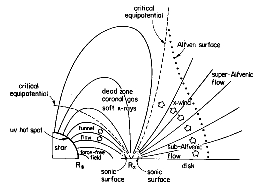
\includegraphics[width=0.9\textwidth]{shu94_3}
\caption{
Shu's X-Wind Model - the jet or x-wind is launched from the R$_x$ region, close to the central object \citep{1994ApJ...429..781S}.
}
\label{fig:XWind} % label
\end{figure}
% Other models
Boundary layer models were proposed by 
\citet{1988ApJ...328L..19S}, \citet{1989MNRAS.236..107P}, \citet{1990RvMA....3..234C} and \citet{1992ApJ...399L.163B}.
The most popular boundary-layer driven model is the X-Wind or X-celerator model.
The X-Wind was model originally propounded by \citet{1988ApJ...328L..19S} as a wind from a rapidly-rotating T Tauri star but extended and modified by \citet{1994ApJ...429..781S,1994ApJ...429..797S,1994ApJ...429..808N}. 
This differs from the previous models in that the magnetic field is argued to be from the protostar rather than an external field threading the disk.
\citet{1994ApJ...429..781S} argue that the disk excludes the magnetic field.
% Weaknesses
\citet{1989MNRAS.236..107P} pointed out that the requirement for the protostar to be spinning at close to breakup is in contradiction with the observations.
The modifications in \citet{1994ApJ...429..781S} allowed for protostars rotating below breakup.
\citet{1992ApJ...387L..47M,1993ApJ...414..230M} found that the X-Wind model could not account for the mass-velocity power-law $m(v) \sim v^{-1.8}$ relation found consistently in CO observations of molecular outflows in L1551 \citep{1988ApJ...332..364M}, NGC 2051 \citep{1988ApJ...332..364M}  and HH46-47 \citep{1991ApJ...382L..93C}.
\citet{1995ApJ...455..182C} found that the X-Wind model could not account for observed momentum distributions.
\citet{1996ApJ...468..261L} addressed the criticisms of \citet{1992ApJ...387L..47M} and modified their model accordingly.
%The X-wind model cannot necessarily be applied to all jets in astrophysics, e.g. AGN jets for example - this is its main weakness.
The main weakness of the X-Wind model is that it is star-formation specific and cannot be applied to active galactic nuclei, which do not have magnetospheres. 
The X-Wind and disk-wind theories are not mutually exclusive - there could be for example a high-velocity component X-Wind in the centre surrounded by a lower velocity disk-wind.

\section{Jets and shocks}
Jets from young stellar objects are seen at optical, ultraviolet and infrared wavelengths thanks to their bright Herbig-Haro knots along their length and their terminating bow shocks.

\subsection{Shocks}
%In general feature a forward shock, a reverse rarefaction expansion fan separated by a contact discontinuity. 
%A shock is a type of propagating disturbance in a medium.
% No it can be still


% Fluid may be described by wave motion
%A wave is a propagating disturbance in a medium.
To understand shocks, a brief exposition of wave theory is given.
\citet{1974whitham} intuitively describes a wave as ``any recognisable signal that is transferred from one part of a medium to another with a recognisable velocity.  The signal may be any feature of the disturbance such as a maximum or an abrupt change in some quantity''.
A single conservation law in one dimension:
\begin{equation}
\frac{\partial u}{ \partial t}
+
 \frac{\partial f\left(u\right)}{ \partial x}
=0
\end{equation}
may be written in the form:
\begin{equation}
\frac{\partial u}{ \partial t}
+
a \frac{\partial u}{ \partial x}
=0
\end{equation}
%with initial conditions
%\begin{equation}
%u(x,0) = u_0(x)
%\end{equation}
$u$ is the signal or wave,
$a$ is the wavespeed.
The curves $\frac{dx}{dt}=a$ are the characteristic curves or characteristics.
If $a$ is a function of $u$, the system is nonlinear.
For a system of conservation laws, which could be for example the hydrodynamic equations or the equations of magnetohydrodynamics,
\begin{equation}
\frac{\partial \mathbf{U} }{ \partial t}
+
A \frac{\partial \mathbf{U}}{ \partial x}
=0
\end{equation}
If $A$ is diagonalizable,
\begin{equation}
\frac{\partial \mathbf{v} }{ \partial t}
+
Q^{-1}AQ \frac{\partial \mathbf{v}}{ \partial x}
=0
\end{equation}
where Q is the matrix of right eigenvectors of the $A$,
$\mathbf{v}$ is defined by $d\mathbf{v} = Q^{-1} d\mathbf{U}$,
the eigenvalues $\lambda_i$ of $A$ are the wave speeds,
$\mathbf{v}$ is the vector of signals or information carried by the waves or characteristic variables,
the curves $\frac{dx}{dt}=\lambda_i$ are the wavefronts or characteristics.
An example of the characteristics for the linearised wave equations is shown in Figure \ref{fig:HDWaves}.
%The characteristics may intersect, when they do a shock is formed.
When characteristics from the same family intersect a \emph{shock} is formed.
When the characteristics diverge, an \emph{expansion wave} or rarefaction is formed.
There is a third possibility, where the characteristics are parallel, entropy waves or contact discontinuities.
% Characteristics
%If the equation which describes a system is known
% Characteristics cross - shock
% Characteristics diverge - rarefaction
Physically, a shock is characterised by a sudden violent abrupt change in pressure, temperature or velocity which happens over a distance so short (depending on the microphysics of the system this may be one mean free path for a collisional gas or one particle gyroradius for a low-density plasma) that it may be approximated as a discontinuous change. 
A shock travels faster than information can propagate though a system, so the medium has no time to react.
Entropy waves or contact discontinuities are characterised by a jump in entropy, where the pressure is constant. Entropy waves may exist as static phenomena, whereas shocks result from dynamic action.
Nonlinear acoustic waves steepen into shocks when they ``break'' like waves on a beach.  
Gas which passes through a shock or which a shock passes through is heated and compressed and cools by radiating energy.
Many astrophysical problems, such as supersonic jets, novas, coronal mass ejections, involve large masses of gas colliding at high speeds. 
In such cases, a mathematical description may be applied by abstracting the situation to a one-dimensional ``shock tube''.


\begin{figure}[t]
\centering
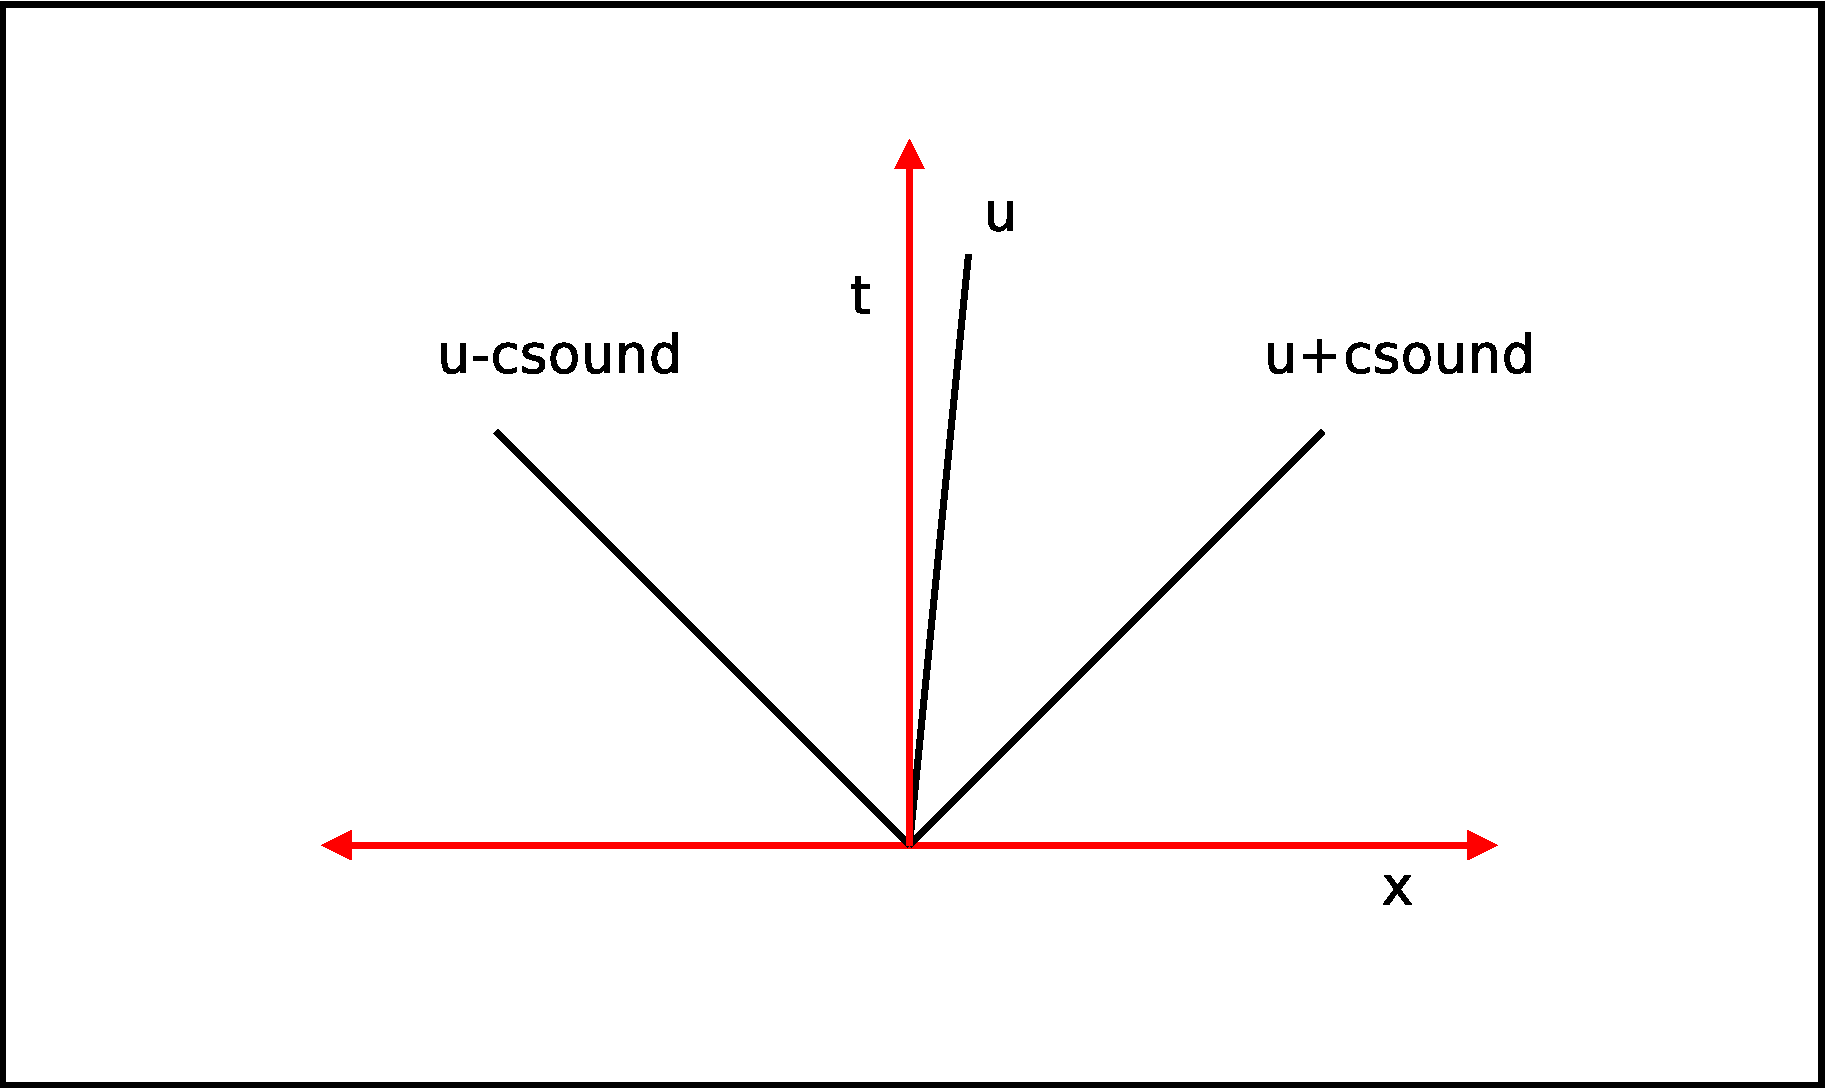
\includegraphics[width=8cm]{HDWaves}
\caption{
The three hydrodynamic waves arising from the breakup of a discontinuity in a fluid in a one-dimensional shock tube. The entropy wave, u, separates the forward-moving shock or rarefaction from the reverse-moving shock/rarefaction.
}
\label{fig:HDWaves} % label
\end{figure}

%In the context of gasdynamics, shocks often accompanied by a contact discontinuity, across which pressure and normal velocity are constant. 
The contact separates the shock from another wave, which may be either compressive (shock) or rarefactions/expansion (see Figure \ref{fig:HDWaves}).
%There are analytical solutions for some shocks e.g. that of B. Riemann for the case of a one-dimensional shock.
In the case of a jet propagating into an ambient medium there is a forward moving shock at the head of the jet (the bow shock) and a reverse shock (Mach disk) separated by a contact discontinuity (slip surface).
Along the length of the jet variations in the velocity of the source produce internal working surfaces which are thought to be the cause of the Herbig-Haro knots.


\begin{figure}[t]
\centering
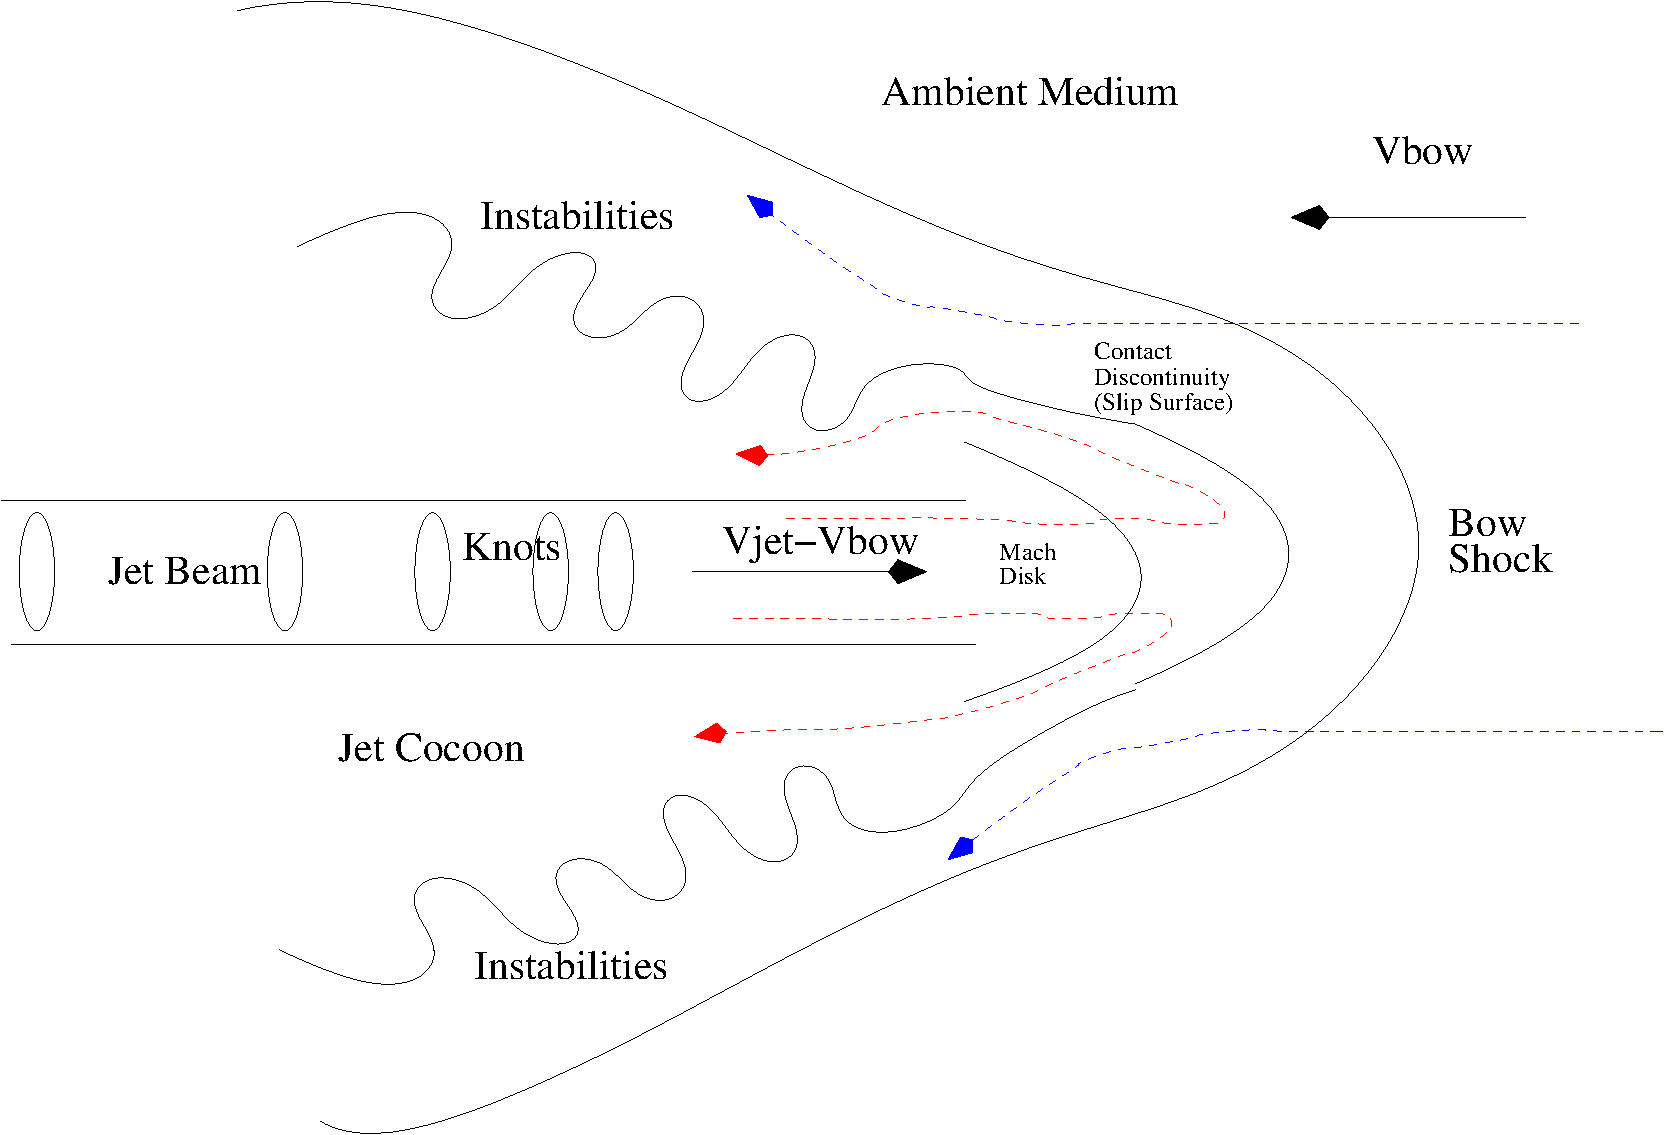
\includegraphics[width=10cm]{JetSchematic}
\caption{
Terminal Working Surface in the rest frame of the shock.
}
\label{fig:WorkingSurface} % label
\end{figure}

%In Figure \ref{fig:WorkingSurface}, a working surface is shown in the rest frame of the contact discontinuity, the ``shock frame''. 
In the rest frame of the contact discontinuity, the ``shock frame''
(see Figure \ref{fig:WorkingSurface})
the bow shock sees the ambient medium approach it with a velocity $V_{bow}$. The jet is incident on the Mach disk with velocity $V_{jet}-V_{bow}$. 
Gas crossing the Mach disk experiences a rapid, unexpected drop in velocity and most of this energy is immediately converted to heat. 
At some surface between the two shocks, the ram pressures of the colliding fluids balance and there is no net transfer of material. 
This surface is the contact discontinuity. 
It is also well described as the ``slip surface'' since the shocked ambient and jet material slips sideways and out into the cocoon. 
The jet and ambient matter can have different shear velocities and generate Kelvin-Helmholtz instabilities.


\subsection{Radiative shocks and ``Forbidden'' line emission}

\begin{figure}[t]
\centering
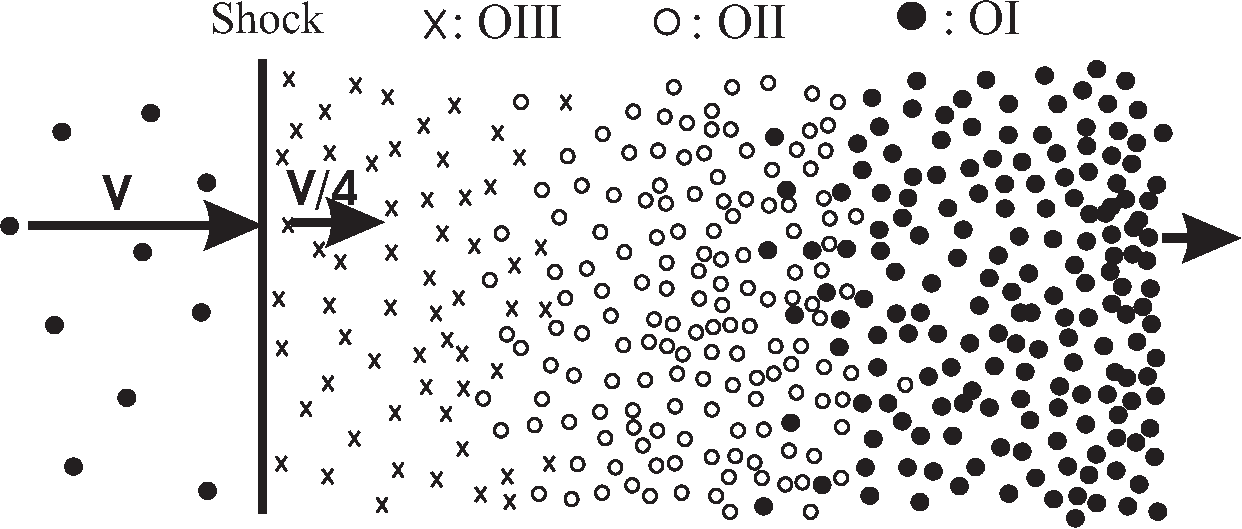
\includegraphics[width=10cm]{redone_shock}
\caption{
Crossing the shock, there is a rapid increase in density. The density then gradually increases as the thermal energy is radiated away. Shown in the figure are the cooling zones of [OIII], [OII] and [OI].
}
\label{fig:RadShock} % label
\end{figure}

%Radiative shocks radiate away thermal energy, thus have a rapid drop in pressure behind the shock (the post-shock region). There is then a thin dense shell behind the shock.

As incoming material crosses the shock it experiences a rapid increase in density.
$ \frac{\rho_{postshock}}{\rho_{preshock}} = \frac{\gamma +1}{\gamma -1}$,
where gamma is the adiabatic index or ratio of specific heats.
For the adiabatic case, $\gamma = 5/3$, the density ratio is 4.
For a radiatively cooling shock, $\gamma$ is effectively lowered and the jump in density can be much  greater.
% Crosses shock
% Increase density
% Increase collisions
% But density still low enough to doesn't collisionally de-excite.
The amount of ionisation and excitation due to collisions is significantly increased in the thin dense ionising/exciting layer at the shock front.
% Atoms will be excited into the metastable states, from which they may have a highly improbable transition to a lower energy level, providing that they do not collide with another atom.
% At 
Radiative transitions which obey the normal electric dipole quantum mechanical selection rules are called ``permitted'' emission lines.
Those which obey the slower magnetic dipole or electric quadrupole rules are called ``forbidden'' lines.
These lines have low transition probabilities (typically 1 s$^{-1}$) compared to
permitted lines \citep[(typically 10$^8$ s$^{-1}$)][]{1980pim..book.....D}. 
% but are highly visible since the interstellar medium is optically thin to the photons they produce.
%If an excited atom does not collide with another and de-excite, there may occur a spontaneous radiative transition not to the ground state, but to an intermediate state. 
%The probability of this occurring is low (1 s$^{-1}$) compared to the probability of an electron collision de-excitation,  
%Although the probability of this occurring is low, photons from such transitions have equally low probabilities of being reabsorbed, so are more likely to be detected far away. Because these low probability transitions are only observed in most of the galaxy and the upper atmosphere, and not on the surface of the Earth, they are referred to as ``forbidden'' transitions.
%Immediately after this layer there is a cooling zone from which most of the radiation is emitted.
%Certain radiative transitions which have an extremely low but non-zero probability occur, the so-called ``forbidden'' lines , which are not normally allowed by the selection rules of quantum mechanics.


\subsection{Magnetohydrodynamic shocks}

\begin{figure}[t]
\centering
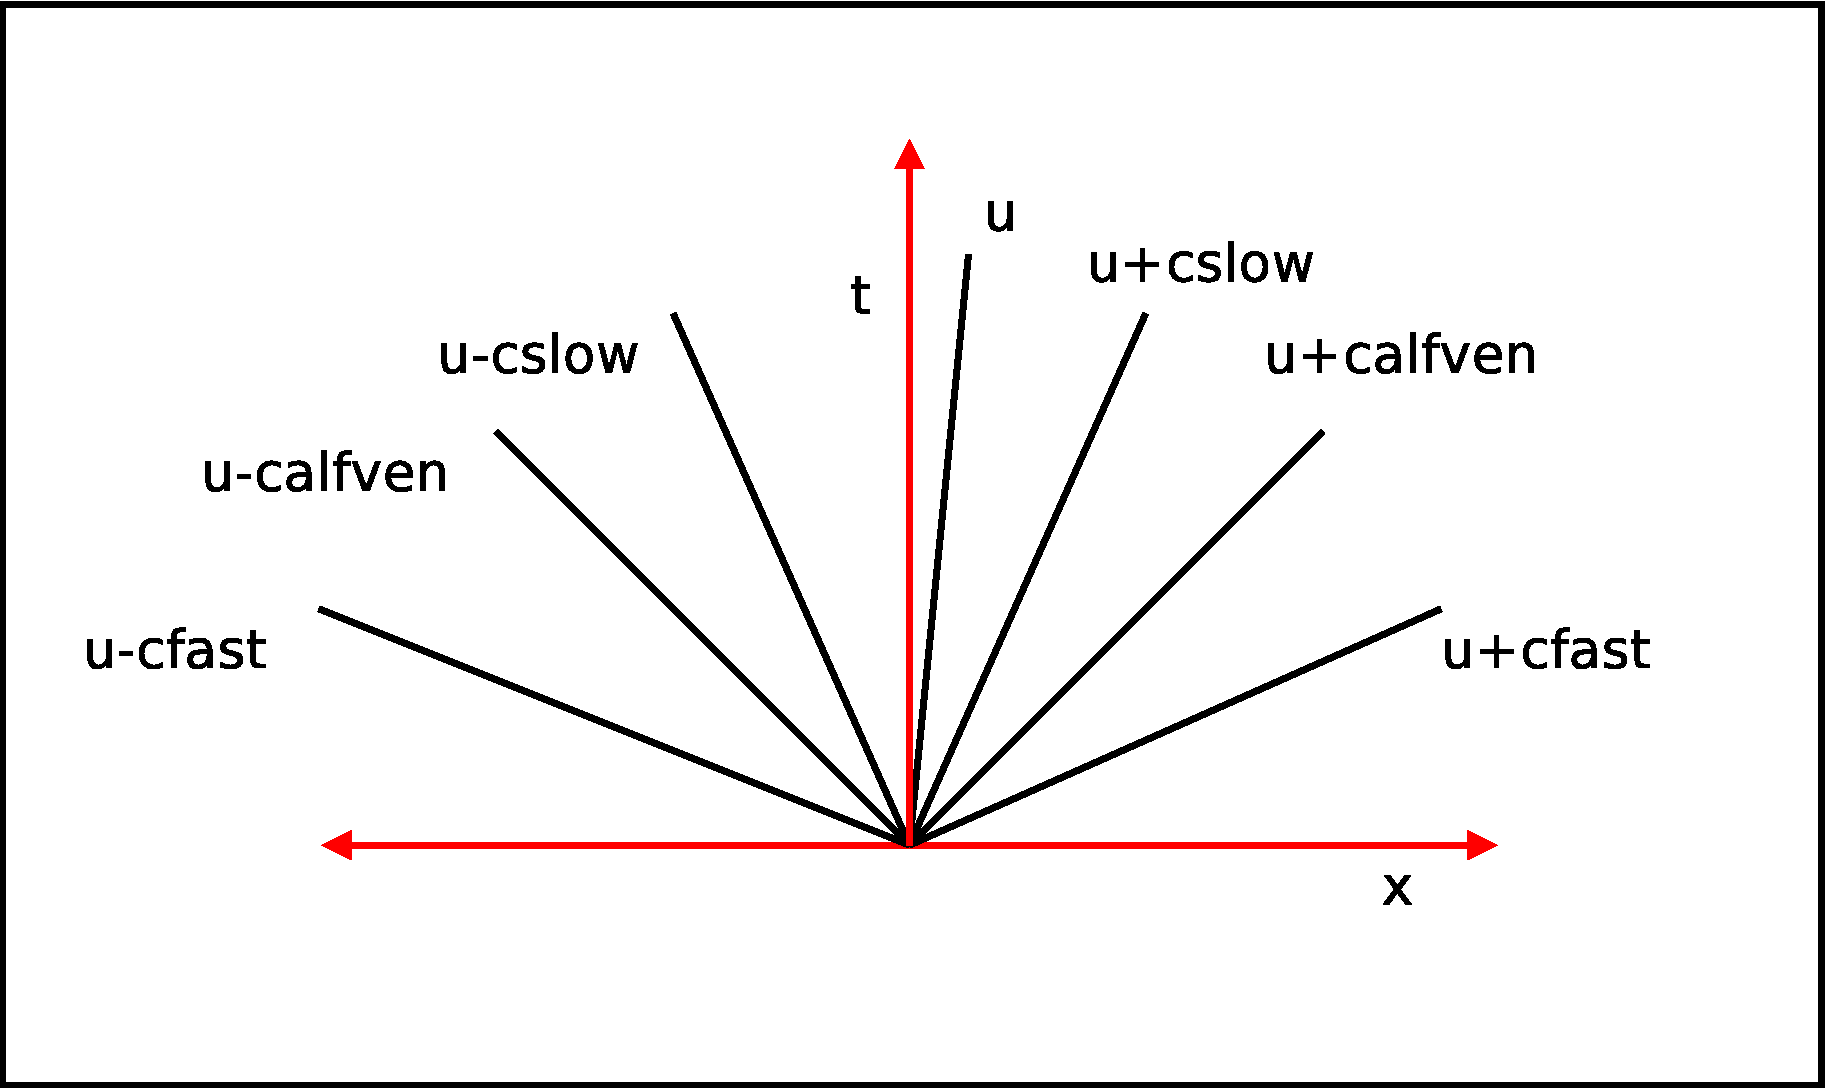
\includegraphics[width=8cm]{MHDSevenWaves}
\caption{
The seven magnetohydrodynamic waves arising from the breakup of a discontinuity in a fluid. The contact wave, u, separates the forward-moving family of slow magnetosonic, Alfv\'en and fast magnetosonic waves from the backward-moving family.
}
\label{fig:MHDSevenWaves} % label
\end{figure}

The magnetic field interacts with the fluid through the Lorentz force.
The Lorentz force, $\mathbf{j}\times \mathbf{B}$, 
can be thought of as affecting the dynamics in two different ways.

\begin{equation}
%\frac{1}{c} \mathbf{J}\times \mathbf{B}= \frac{1}{4 \pi} \left( \mathbf{B} \cdot \boldsymbol{\nabla} \right) \mathbf{B} - \boldsymbol \nabla \left( \frac{B^2}{8 \pi}\right)
 \mathbf{J}\times \mathbf{B}= \frac{1}{\mu} \left( \mathbf{B} \cdot \boldsymbol{\nabla} \right) \mathbf{B} - \boldsymbol \nabla \left( \frac{B^2}{2 \mu}\right)
\end{equation}

The first term represents a \emph{magnetic tension} which acts along the
magnetic field lines, resulting in a transverse wave mode (Alfv\a'{e}n waves).
This is a restoring force analogous to the tension in a violin string. The
Alfv\a'{e}n wave speed is $c_A = \frac{  B_{\perp} }{ \sqrt{\rho}}$.
The second term represents a \emph{magnetic pressure} gradient which can add to or subtract from the ram pressure resulting in the fast or slow magnetosonic wave modes. This has the same dimensional form as the thermal pressure term in the hydrodynamic equations.
Instead of three waves there is a family of seven waves (see Figure \ref{fig:MHDSevenWaves}).
The contact discontinuity remains the same but the forward and reverse moving waves have each been replaced by the set of slow, Alfv\a'{e}n and fast waves.
In a weak or absent magnetic field the Alfv\a'{e}n and slow velocities are zero and the fast velocity collapses to the sound speed.


\subsection{Jump-type (``J-type'') shocks}
In a J-shock the velocity is sufficiently high to exceed the Alfv\a'{e}n velocity, hence there is a jump discontinuity in all the state variables.

\subsection{Continuous-type (``C-type'') shocks}

\begin{figure}[t]
\centering
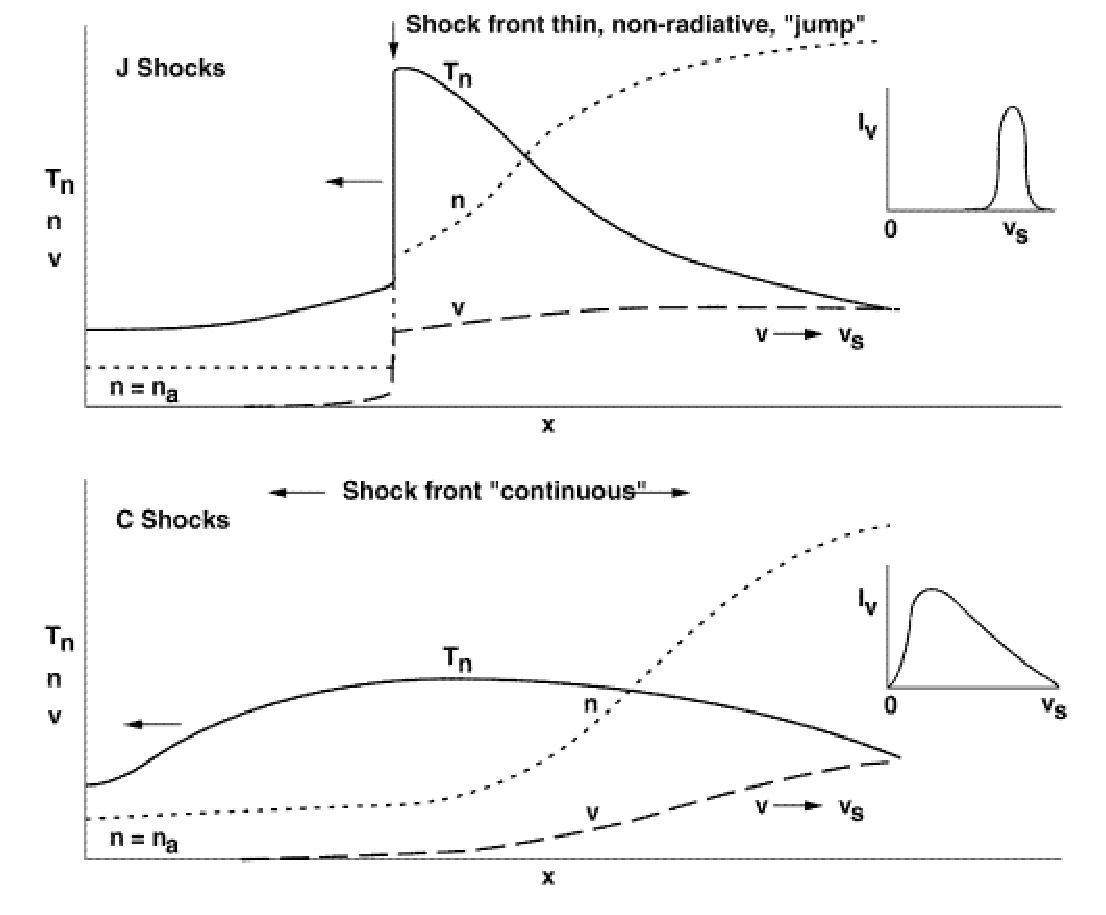
\includegraphics[width=\textwidth]{CJShock}
\caption{
%CShocks and JShocks
Jump-type Shocks and Continuous-type Shocks 
, $T_n$ denotes the neutral temperature, n denotes the neutral number density. v denotes the velocity.
}
\label{fig:CJShock} % label
\end{figure}

\citet{1971MNRAS.153..145M} showed magnetised weakly ionised shocks may have continuous solutions for $v_S$ less than a critical value.
\citet{1980ApJ...241.1021D} introduced the nomenclature ``C-type shock'' to denote weakly ionised shocks where the ion Alfv\a'{e}n velocity $c_A$ exceeds the shock speed, $v_S$. 
In a C-type shock the variables change continuously across the shock, since a magnetic precursor gives the material in the path of the shock time to react to the shock and dissipate its energy smoothly.
The magnetic field has a ``cushioning'' effect; it absorbs some of the incoming momentum.
This can occur when the Alfv\a'{e}n speed is higher than the propagation speed.
This means that not all material is thermalised when it crosses the shock.
But the Wardle instability may cause the C-type shock to be unstable 
for some modal range of magnetic field perturbations
\citep{1997ApJ...487..271S}. 
See \citet{1993ARA&A..31..373D} for a review article.

\subsection{Bow shocks and Internal Working Surfaces}
At the end of the jet a terminating bow shock is formed where the jet ploughs into the ambient gas around it. 
Internal working surfaces appear along the length of the jet - they were
initially thought to be the crossing shocks which appear in jet simulations.
Later they were attributed to velocity variations in the source, which are still
of unknown origin. The latter are thought to result from the reconnection of the
wound up magnetic field. %\citep{}.




\subsection{Jet diagram}


\begin{figure}[t]
\centering
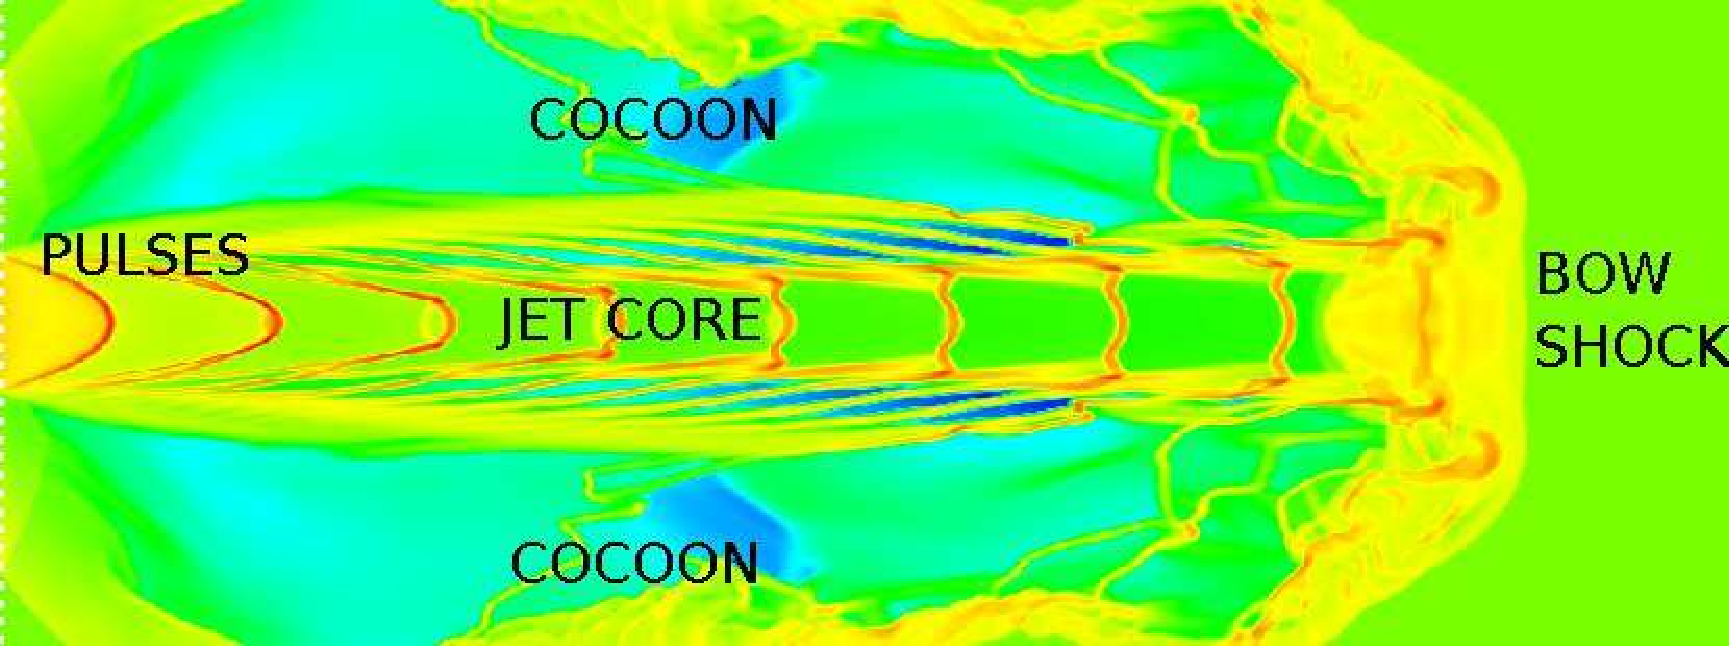
\includegraphics[width=\textwidth]{jet_diagram}
\caption{
Basic features of a radiatively cooling jet - bow shock, internal working surfaces and cocoon.
}
\label{fig:JetDiagram} % label
\end{figure}

In Figure \ref{fig:JetDiagram}, a time-dependent simulation of a radiatively cooling jet is shown.
The dense jet material is injected in at the left side of the box and the velocity is varied, causing the internal working surfaces to form. The internal working surfaces develop instabilities as they progress down the jet core and shed vortices adding to the mixing layer in the cocoon. At the front of the jet the terminal working surface or bow shock ploughs into the ambient medium supersonically. 
%The instabilities caused by the radiative cooling and the velocity variations are clear.

Using a simple one-dimensional approximation, a simple analytic estimate of the bow shock speed is obtained in terms of the jet speed and the ratio of the jet and ambient material densities (assuming ram pressure balanced at the contact discontinuity), which is useful as a simple check on the validity of the numerical simulations.
In the rest frame of the working surface, the ambient medium is
travelling backwards into the surface at a velocity -W, and the jet is
travelling forward at a velocity $v_b-W$. Balancing the ram pressures ${\rho}_b
{(v_b-W)}^2 = {\rho}_a\left( {-W}^2\right)$ leading to $ \frac{v_b}{W}=\frac{\sqrt{\eta}}{1+\sqrt{\eta}} $, where $\eta={\rho}_a/{\rho}_b$.
%Hence, in this work study shocks from jets around protostars using the MHD approximations and by numerical means.
Although this is only a two-dimensional simulation, the thin dense shell of material is clearly unstable and already starts to break up. 
Vortices are shed from the edges of the Mach disk and add to the mixing layer.


\section{From the kinetic theory to MHD}
%How to model all of this?}
% A broad sketch of the outline of the derivation of the MHD equations from kinetic theory
\subsection{Boltzmann's Equation}
The motions of the gas particles may be described by the Boltzmann kinetic equation.

\begin{equation}
\frac{D{f}}{D{t}}=
\frac{\partial{f}}{\partial{t}}
+
\mathbf{v}
\cdot
{\boldsymbol{\nabla}}_x f
+
%\frac{q}{m}
%\left(
%\mathbf{E}
%+
%\frac{\mathbf{v}\times \mathbf{B}}{c}
%\right)
\mathbf{a}
\cdot
{\boldsymbol{\nabla}}_v f
=
\left( \frac{\partial{f}}{\partial{t}} \right)_{collisional}
\end{equation}
where $f$ is the single-particle distribution function in phase space (the probability to find a particle at point $\mathbf{x}$ travelling at $\mathbf{v}$ at a time t), $f(\mathbf{x},\mathbf{v},t)d^{3}x d^{3}v$ is the number of particles within an interval in phase space at time $t$.
$\mathbf{v}$ is the total velocity (bulk and random components).
$\mathbf{a}$ is the acceleration term, which represents the contribution made by external resultant forces such as gravity, $\mathbf{g}$ or the electromagnetic force $\left(\frac{q}{m} \left( \mathbf{E + u \times B}\right)  \right)$.  

% Collisions cannot contribute
Since collisions cannot contribute to the change of quantities such as mass,
momentum and energy, whose total is conserved in the collisional process, the
left-hand side becomes the collisionless Boltzmann or Vlasov equation.

\begin{equation}
\frac{\partial{f}}{\partial{t}}
+
\mathbf{v}
\cdot
{\boldsymbol{\nabla}}_x f
+
%
%\frac{q}{m}
%\left(
%\mathbf{E}
%+
%\frac{\mathbf{v}\times \mathbf{B}}{c}
%\right)
\mathbf{a}
\cdot
{\boldsymbol{\nabla}}_v f
=0
\end{equation}

Substituting $n \langle Q \rangle $ for $f$, where $ \langle Q \rangle = n^{-1} \int Q f d^3v $
gives

\begin{equation}
\frac{\partial{ n \langle \chi \rangle }}{\partial{t}}
+
 {\boldsymbol{\nabla}}_x n{\langle \mathbf{v} \chi \rangle}
+
n
\langle
\left(
\mathbf{a} \cdot
{\boldsymbol{\nabla}}_v
\right)  { \chi }
\rangle
=0
\end{equation}
%wind
where $\chi$ represents a conserved quantity such as mass, total energy or momentum.

\subsection{Moment Equations}
In this system, $\mathbf{x},\mathbf{v}$ and t are all independent variables.
In order to simplify the system, velocity, $\mathbf{v}$ may be removed by taking moments of the Vlasov equation.
This results in an infinite chain of equations.
After taking the zeroth, first and second moments the series may be truncated by the addition of a closure equation or equation of state.

\begin{equation}
\left( 
\begin{array}{c}
\rho \\
\rho u \\
E 
%\rho \epsilon
\end{array}
\right) 
=
\int
{
\left( 
\begin{array}{c}
m \\
m\mathbf{v} \\
m\left| \mathbf{v} \right| ^2 /2
\end{array}
\right) 
f(\mathbf{x},\mathbf{p},t)
}
d^3v
\end{equation}

\subsubsection{Zeroth Moment: The Continuity Equation}
Taking the zeroth moment, $\chi = m $, gives 
\begin{equation}
\frac{\partial \rho}{\partial t}+\boldsymbol{\nabla}\cdot(\rho \mathbf u)=0
\end{equation}
The familiar continuity equation, expressing the conservation of mass and the fact that it changes in a continuous fashion.


\subsubsection{First Moment: The Momentum Equation}
Taking the first moment, $\chi = m \mathbf{v} $, gives 

\begin{equation}
\frac{\partial{ n \langle m \mathbf{v} \rangle }}{\partial{t}}
+
\mathbf{v}. {\boldsymbol{\nabla}}_x n{\langle m \mathbf{v} \rangle}
+
n
\langle
\mathbf{a} 
{\boldsymbol{\nabla}}_v . { m \mathbf{v} }
\rangle
=0
\end{equation}
Dividing $\mathbf{v}$ into bulk and random components $\mathbf{v=u+w}$,
gives 

\begin{equation}
\langle \mathbf{v} \rangle= \langle \mathbf{u} \rangle
\end{equation}
and 
\begin{equation}
\langle \mathbf{v v} \rangle= \langle \mathbf{u u} \rangle + \langle \mathbf{w w} \rangle
\end{equation}
$ \rho\langle \mathbf{w w} \rangle$ is defined as the pressure tensor. It may be divided into an isotropic gas pressure and a viscous stress tensor.
$ \rho \langle \mathbf{w w} \rangle = P{\overline{ \overline I} } + {\overline { \overline \pi}} $,
where 
\begin{equation}
P = \rho \frac{1}{3} {\left| \mathbf{w} \right|}^2
\end{equation}
\begin{equation}
{\overline {\overline \pi}} = \rho \frac{1}{3} {\left| \mathbf{w} \right|}^2 - \rho \langle \mathbf{w w} \rangle
\end{equation}
Assuming the fluid is inviscid ${\overline {\overline \pi}}=0$.
\begin{equation}
\frac{\partial}{\partial t}\left(
\rho \mathbf u
\right)
+ {\boldsymbol{\nabla}}_x
\cdot
\left( 
\rho 
\mathbf {u} \otimes \mathbf{u} 
+
P{\overline{ \overline I} }
\right)
+ \rho \mathbf{a}
=0
\end{equation}
This equation describes the conservation of momentum.

\subsubsection{Second Moment: The Total Energy Equation}

Taking the second moment, $\chi = m {\left|v\right|}^2 $, gives 
\begin{equation}
\frac{\partial}{\partial t}E
+
{\boldsymbol{\nabla}}_x 
\left( 
\mathbf{u} \left( E +P \right)
\right)
+
\rho \mathbf{u} \mathbf{a}
=0
\end{equation}
The derivation is straightforward, but involves several steps - it is therefore relegated to Appendix \ref{MHDDerivation}.
This equation describes the conservation of energy.
%The equations may be derived by taking zeroth, first and second velocity moments of the collisionless Boltzmann or Vlasov equation.

%However this is too large a system to be solved directly and thus certain assumptions are made which the use of fluid approach and a reduced form of Maxwell's equations - the equations of magnetohydrodynamics.
%Rather than directly solving the Boltzmann equation - make the assumptions of fluid dynamics and MHD, and include the non-ideality of optically thin atomic radiative cooling losses.

\subsection{Maxwell's Equations}

The $\mathbf{a} $ term contains all the acceleration provided by gravitational and electromagnetic forces. The electromagnetic forces are described by Maxwell's equations.

% xxxxxxxxxxxxxxxxxxxx
\begin{eqnarray*}
\boldsymbol{\nabla} \cdot\mathbf{D} &= & {\delta}_Q \\
\boldsymbol{\nabla} \cdot\mathbf{B} &=&0 \\
\boldsymbol{\nabla} \times\mathbf{E} &=& -\frac{\partial \mathbf{B}}{\partial t} \\
\boldsymbol{\nabla} \times\mathbf{H} &=&  \mathbf{J}+ \frac{\partial \mathbf{D}}{\partial t}
\end{eqnarray*}
$\mathbf{H}$ is the magnetic field strength.
$\mathbf{D}$ is the electric flux density.
${\delta}_Q$ is the charge density.
$\mathbf{B}$ is the magnetic field intensity.
$\mathbf{E}$ is the electric field intensity.
$\mathbf{J}$ is the current density.
$\mathbf{B} = \mu \mathbf{H}$, where $\mu$ is the magnetic permeability.
$\mathbf{D} = \epsilon \mathbf{E}$, where $\epsilon$ is the electric permittivity.

%The goal is to model the shocks from jets and outflows from YSOs (described by Boltzmann's equation), taking into account magnetic fields (described by Maxwell's equations) and loss of thermal energy due to optical thin radiation.
% Is the fluid approach valid

\subsection{Quasi-Neutral Single Fluid Approximation}

In order to solve Maxwell's equations and the equations of fluid dynamics it is first necessary to make the approximations of MHD.
The assembly of particles (ions, electrons and neutrals) can be approximated as a fluid, if the mean free path is much smaller than the length scale of interest.
\begin{equation}
\lambda_{mfp} << L_{char}
\end{equation}
Viscosity is assumed to be zero (high Reynolds number) 
\begin{equation}
\eta \sim 0 \rightarrow Re= \sim \infty
\end{equation}
The particles are collisionally coupled.
The system can be simplified from the multiple fluids (electrons, ions of different species) to a single fluid approach if it assumed that charged particles are coupled to neutrals.
The length scale of interest is 10$^{15}$ cm, whereas the mean free path $l=(n\sigma)^{-1}$ is  $l=10^{13}$ cm (for cross-sectional area $\sigma_{csa} = 10^{-15}$ cm$^{-2}$ and $n=10^2$ cm$^{-3}$).
It is further assumed that electrons and ions do not show a Hall separation and that the neutrals do not exert a drag on the charged particles.
%the gas is near equilibrium, pressure is isotropic, 
% Are the assumptions of MHD valid
% what are the assumptions of MHD?
Assuming quasi-neutrality (the charge density, $\delta_Q$ is zero). 
\begin{equation}
\delta_{Q} = 0
\end{equation}
Due to electrostatic attraction, each charged particle will be surrounded by other oppositely charged particles which will screen it (Debye screening). The radius at which the electrostatic force is negligible is the Debye-H\"{u}ckel length. 
\begin{equation}
L_D^{-2} \equiv \frac{4\pi e^2}{kT}(n_e+{Z_i}^2 n_i)
\end{equation}
%Infinite conductivity is assumed, 
%\begin{equation}
%\sigma_c >> 1
%\end{equation}
%the heat flow can be neglected, 

\subsection{Ideal MHD Approximations}

Following \citet{1975clel.book.....J}, the displacement term in the Amp\a`{e}re-Maxwell law may be neglected, 
\begin{equation}
\boldsymbol{\nabla}
\times
\mathbf{B}
= 
\mu
\mathbf{J} +
\mu
\frac{\partial \mathbf{D} }{\partial t} 
\end{equation}
Taking the equations:
\begin{equation}
\boldsymbol{\nabla}
\times
\mathbf{B}
= 
\mu
\mathbf{J} 
\end{equation}

\begin{equation}
\boldsymbol{\nabla}
\times
\mathbf{E}
=
-
\frac{\partial \mathbf{B} }{\partial t} 
\end{equation}
Substituting in for $\mathbf{E}$ using Ohm's law $ \mathbf{J}=\sigma (\mathbf{E} + \mathbf{u}\times\mathbf{ B}) $, where 
$\mathbf{J}$ is the current density and
$\sigma$ is the conductivity
 (and neglecting along the way the Joule dissipative term and the pressure gradient term from the generalised Ohm's law) - one obtains:
\begin{equation}
\frac{\partial \mathbf{B} }{\partial t} 
+ 
\boldsymbol{\nabla}
\times
\left(
\mathbf{B}
\times
\mathbf{u}
\right)
-
\frac{1}{\mu \sigma}
\boldsymbol{\nabla}
\times
\left(
\boldsymbol{\nabla}
\times
\mathbf{B}
\right)
=
0
\end{equation}
For a stationary fluid letting $\mathbf{u}=0$ and applying $\boldsymbol{\nabla} .\mathbf{B} =0$ this reduces to
\begin{equation}
\frac{\partial \mathbf{B} }{\partial t} 
=
\frac{1}{\mu \sigma}
{\boldsymbol{\nabla}}^2 \mathbf{B}
\end{equation}
%can neglect the high-frequency components of the electric field, 
%and that the number density is proportional to the mass density.
- a standard diffusion equation in which the field decay time is as follows:
\begin{equation}
\tau =  \mu \sigma L^2
\end{equation}
and this is effectively infinite (about 10$^{10}$ years) given large scales in astrophysical systems and high conductivity, 
Hence with high conductivity, magnetic Reynolds number $R_M =V \tau / L$
and magnetic field decay diffusion time are effectively infinite and magnetic lines of force are effectively ``frozen" into the fluid.
%\begin{equation}
%R_M =\frac{ V \tau}{ L}
%\end{equation}
Alfv\a'en's Theorem (1943): ``In a perfectly conducting fluid $ R_m \rightarrow \infty $, magnetic field lines move with the fluid: the field lines are `frozen' into the plasma." 
The induction equations is then reduced to just two terms:
\begin{equation}
\frac{\partial \mathbf{B} }{\partial t} 
+ 
\boldsymbol{\nabla}
\times
\left(
\mathbf{B}
\times
\mathbf{u}
\right)
=0
\end{equation}

This equation implies $ \frac{d}{dt} \int_\mathbf{S} \mathbf{B}.d\mathbf{S} =0 $
which implies that the flux, $\mathbf{B}$,
threading a surface, $\mathbf{S}$, does not change as $\mathbf{S}$  moves through the
fluid. See  \citet{1998pfp..book.....C} or many standard texts for a proof of this.

\subsection{Rankine-Hugoniot Conditions}


The ideal magnetohydrodynamics (MHD) equations are a simplified model used to describe the behaviour of a magnetised fluid over time and space. They are coupled non-linear vector differential equations.
They express the conservation laws, of mass, momentum, magnetic flux density, and energy. 
The approximations of MHD break down once in the shocked regime, however the conservation laws still apply. 
When one applies the conservation laws across a shock, the Rankine-Hugoniot conditions for shocks can be derived. 
\citet{1950PhRv...80..692D} derived the Rankine-Hugoniot jump conditions for the magnetohydrodynamic case.

\begin{eqnarray*}
s [\rho]&=& [\rho u_x] \\
s [\rho u_x]&=& [\rho u^2 + P -\frac{1}{2}{B_x}^2] \\
s [\rho u_y]&=& [ \rho u_x u_y - B_x B_y] \\
s [\rho u_z]&=& [\rho u_x u_z - B_x B_z] \\
s [B_y]&=& [u_x B_y - B_x u_y]\\
s [B_z]&=& [u_x B_z - B_x u_z]\\
s [E] &=& [ u_x \left( E + P\right) -B_x\left( \mathbf{v \cdot B} \right)] \\
\end{eqnarray*}
The Rankine-Hugoniot Jump Conditions, where
$s$ is the shock speed, $\rho$ is the density, $u_{x,y,z}$ the velocity components, $B_{x,y,z}$ the magnetic field, E the energy and P = $p_{thermal} + \frac{1}{2}\mathbf{B}^2 $ the total pressure.
A jump in a quantity is denoted square brackets
\begin{equation}
[x] = x_1 - x_2
\end{equation}


\section{Numerical methods for solving equations}
%How to numerically solve equations?}

\begin{figure}[t]
\centering
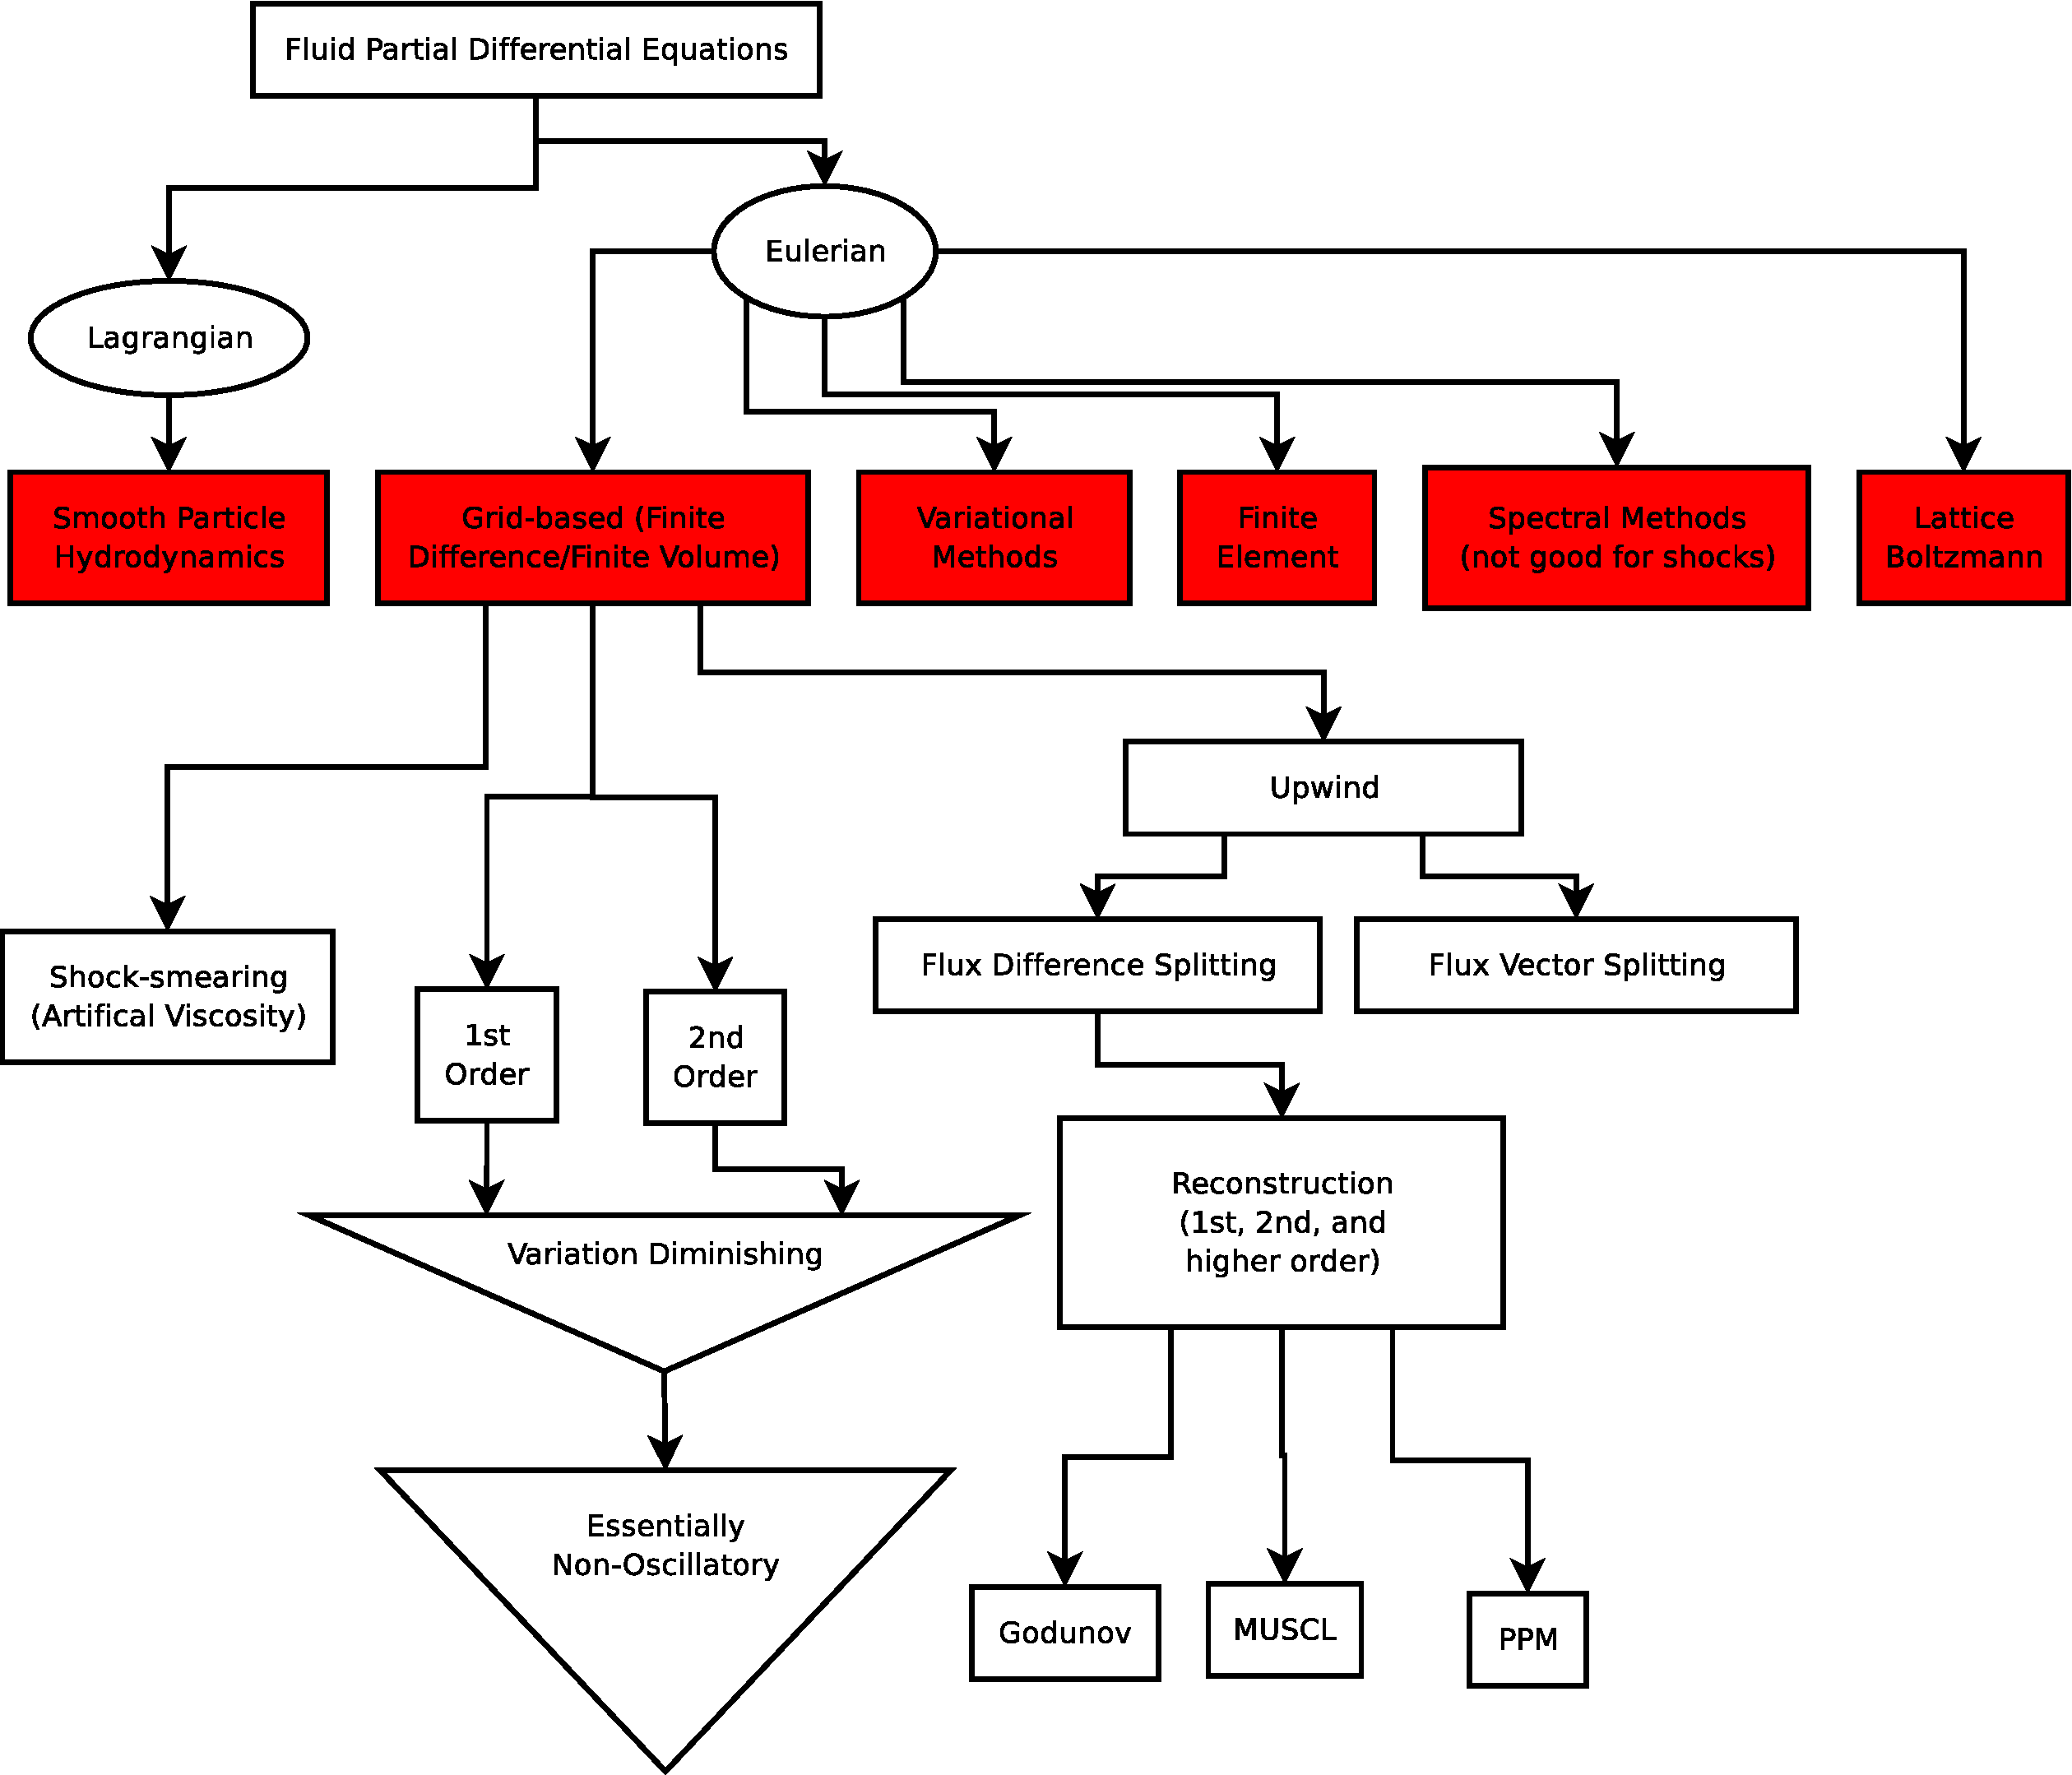
\includegraphics[width=15cm]{NumericalMethodsforTheFluidEquations}
\caption{ 
Numerical methods for solving the fluid partial differential equations
}
\label{fig:NumMeth} % label
\end{figure}

The evolution of an astrophysical gas is described by a set of coupled hyperbolic differential equations, the MHD equations.
These equations are nonlinear, have no general analytical solution and in most cases must be solved numerically.
Numerical solutions can be found using a large number different of schemes.
In fact, numerical models are depicting jets in nature more and more accurately as more and more physics can be included (see section \ref{StateOfTheArt}).
One initial choice that can be made is to solve the equations in a fixed reference frame with a moving fluid (Eulerian) or a moving reference frame (Lagrangian).
In many codes, the physical fluid is represented on a grid of cells with values at the cell centres and cell faces.
This representation, where the co-ordinate system does not co-move with the fluid is called the Eulerian representation.
%It is evolved in time using a numerical scheme.
% First order
% second order
% conservative
% upwind
% implicit explicit

Existing schemes span a range of types from simple first-order schemes (e.g. Lax-Friedrichs) which,
while perfectly adequate for smooth initial conditions,
can smear the solutions of shocked initial conditions so common in modern astrophysical applications,
to second-order schemes which often can capture steeper gradients at the expense of numerical oscillations (e.g. Lax-Wendroff),
to high-order schemes which attempt to capture shocks with a minimum amount of approximation,
to implicit schemes, e.g. Crank-Nicholson, which are computationally intensive
and complex but have stability advantages,
to essentially non-oscillatory schemes,
finite element,
spectral methods,
and 
variational methods.

Shocks are typically represented by steep gradients which, because the equations are non-linear, can cause simple second-order schemes to become rapidly unstable. 
To avoid instability a scheme based on an analytical solution which does exist is used - the Riemann solution to the shock tube problem.
This is a self-similar solution for two uniform states of a fluid. 
By treating every boundary between two neighbouring cells as a one-dimensional Riemann problem, and solving either analytically or approximately, a solution can be spliced together.

Astrophysical problems on a large scale require a large amount of computational
power and an efficient use of limited available facilities. More efficient use
of available computational power can be made by concentrating on areas in the
computational domain where changes are taking place and neglecting those where
the solution is stationary over time. This can be achieved by using an adaptive
mesh, which can refine the grid when the gradients become steep (where the
physics is changing) and derefine the grid where high resolution is unneeded
(where the solution is not changing).


For sufficiently large problems, especially three-dimensional, a single desktop PC is not sufficient to find a solution in a reasonable length of time.
Performing a simulation in 3D, with for example 64x64x128 cells, even using adaptive mesh refinement to cut down on number of calculations required already exceeds the specifications of most PCs and requires the use of a parallel machine.
Problems must be solved in parallel using a large number of machines, either with a shared-memory architecture or a distributed memory architecture.

\subsection{History and current state of star formation jet simulations}
\label{StateOfTheArt}
% History and background of jet models
% Cooling
% Kelvin-Helmholtz
% MHD
% Chemistry
% Jet launching
Numerical models of optical jets have evolved over the past twenty years as the understanding and interpretation of observations increased. 
Most of the early jet simulations were of extragalactic jets.
% Norman 81 - the first hydro jet simulations
Early simulations were by \citet{1981ApJ...247...52N} of the \citet{1974MNRAS.169..395B} twin-exhaust model. These were hydrodynamic slab-symmetric models which displayed the basic features of bow shocks, crossing shocks and cocoons.
% First YSO jet simulations
\citet{1983ApJ...274..677P} and \citet{1986ApJ...301..571P} applied the methods of \citet{1981ApJ...247...52N} to protostellar jets.
% Clarke 86 first MHD jet sims
Magnetic fields were introduced by \citet{1986ApJ...311L..63C}. They used a toroidal field and advected the magnetic vector potential rather than the field strength in order to preserve $\boldsymbol{\nabla} \cdot \mathbf{B} =0$.
% Raga 87 first cooling 
One of the major physical differences between AGN jets and jets from young stars is the amount of cooling due to atomic and molecular processes.
Atomic radiative cooling was introduced by
\citet{1984ApJ...276..560H}, \citet{1987ApJ...316..323H} and \citet{1988ApJ...326..323R} using 1.5D bow shock models which explicitly tried to model observed features.
% Blondin 90
\citet{1990ApJ...360..370B} used an approximation to young stellar object parameters for radiatively cooling jets.
% First use of Riemann solvers
A major step forward was made by \citet{1988JCoPh..75..400B} who derived an approximate Riemann solver for MHD. Now Godunov methods could be applied to astrophysical jet simulations.
% Raga 90 velocity variations
Time variations in the jet velocity were used by \citet{1990ApJ...364..601R}
to explain the knots in Herbig-Haro objects.
% Falle 91
% Stone 92
% Falle 93 AMR % Klein 94 first AMR 
In order to increase the amount of resolution in the physically interesting regions, 2D local adaptive mesh refinement codes were applied to gas dynamics by \citet{1993MNRAS.261..573F} and \citet{1994ApJ...420..213K}.
% Falle 95
% Raga 95 - first molecular cooling
\citet{1995A&A...296..833R} introduced molecular cooling into jet simulations.
% Rosen Smith - molecular cooling
% de Gouveia dal Pino 93 first MHD cooling
3D SPH models were performed by \citet{1993ApJ...410..686D} which were the first jets to be both magnetised and include radiative cooling losses.
% Frank 98 
% Lim first chemical networks
\citet{1999MNRAS.308.1126L} added chemical networks for the first time.
% Truelove 98 - Lim 2000 - 3D AMR 
3D adaptive mesh refinement codes were applied to gas dynamics by \citet{1998ApJ...495..821T} and \citet{2001MNRAS.322..166L}.
% Gardiner 99
% O'Sullivan 2000 - axi MHD jets
% Klein 2003 -AMR 
% Raga 2005 chemistry
%The field has since progressed to more complicated geometries and physics including atomic radiative cooling \citet{1998AJ....116.2943R,2000A&A...364..763R,2001A&A...367..959R}.
The state of the art jet simulation is now fully three-dimensional, with
molecular and atomic cooling, adaptive mesh refinement, magnetic field and
sometimes chemical networks and radiative transfer included.



\section{Structure of this thesis}


In this thesis the propagation of magnetised radiative jets from binary sources, and the propagation of jets in evacuated cavities is studied. For these studies a new numerical code is used.

In Chapter 2 the numerical methods used and the numerical code are introduced. 
In Chapter 3 the code is rigorously tested and compared against the results of other investigators. 

In Chapter 4 the binary jet model is explored. 
% Outflows and jets seem to appear in almost every forming star that has been observed.
Molecular outflows and jets are near ubiquitous in the star formation process.
% Lots of Binaries
%
Multiplicity is a similarly identifiable trend as a large majority of stars appear to form in binaries or multiple star configurations.
% Why no binary outflows?
The question is then: why are most outflows not visibly binary outflows?
% Let's model binary jets and show they don't stay binary for long
%Detailed numerical modelling of binary jets can show that it is physically possible for them to not remain as binaries.
% by launching jet simulations
A time-dependent model of a binary jet system can be used to examine the effects of source orbiting, magnetic fields and jet interaction on the morphology and propagation of the jets.
Therefore numerical simulations of the two jet model are performed and the MHD parameters are based on observations of a specific object, LDN1551 IRS 5 (HH154).


In Chapter 5 the relationship between a jet and its environment is examined. The propagation of jets in evacuated cavities is investigated. 
The idea of a density gradient allowing the jet from a protostar to collimate has a venerable history, stretching back to 
\citet{1974MNRAS.169..395B},
\citet{1982ApJ...261..115K},
\citet{1982PASJ...34..483F},
\citet{1984Ap&SS..98..315S},
\citet{1984ApJ...277L..35F}
and
\citet{1986PASJ...38..199O}.
Jets are collimated, episodic phenomena which possess a prehistory of outflows moulding the molecular cloud. In the current study a firm connection between a jet and its established prehistoric environment is demonstrated. Herbig-Haro jet phenomena are remarkable for
their high velocities and unusually collimated morphologies, extending
up to parsec scales with opening angles of $0-3^{\circ}$
\citep{2000prpl.conf..815E}. The physical cause of the collimation is
as yet undetermined however major influences may be the environment in
the immediate vicinity of the source and the prehistory of multiple
episodic outflows from the same source. Close to sources, observations
have shown strong energetic emission and strong ionisation, as measured
by the ionisation fraction \citep{1999A&A...342..717B}. One potential
source could be strong shocks due, for example, to recollimation.

%In Chapter 6 some additional research in the star formation area is presented.
%In Chapter 6 the theme of the star forming environment is extended to the entire
%Galactic Plane.
%In order to know the morphology of star-formation regions, dust is used to trace the molecular clouds.
%The distribution of dust in the Galaxy is studied, using another new code to compute accumulated star counts at different magnitudes, and calculate the extinction. Star forming areas are mapped using a distributed computing system or ``grid''.

Finally, conclusions are drawn and future work is mapped out.
